% PhotonWeave lab-meeting slides.
% Compile with XeLaTeX (Korean text): xelatex photonweave-lab-meeting.tex
% Figures are built by: python docs/presentation/make_figures.py
\documentclass[aspectratio=169,11pt]{beamer}

\usetheme{metropolis}
\metroset{numbering=fraction, progressbar=frametitle, block=fill, sectionpage=progressbar}

\usepackage{fontspec}
\usepackage{kotex}
\usepackage{graphicx}
\usepackage{booktabs}
\usepackage{array}
\usepackage{amsmath}
\usepackage{tikz}
\usepackage{listings}
\usetikzlibrary{arrows.meta, positioning, calc, fit, backgrounds, shapes.geometric,
                decorations.pathreplacing, patterns, shadows.blur}

% ---------------------------------------------------------------- fonts ----
% Korean text falls back gracefully when a font is missing on another machine.
\IfFontExistsTF{NanumBarunGothic}{%
  \setmainhangulfont{NanumBarunGothic}\setsanshangulfont{NanumBarunGothic}}{%
  \IfFontExistsTF{NanumGothic}{\setmainhangulfont{NanumGothic}\setsanshangulfont{NanumGothic}}{}}
\IfFontExistsTF{NanumGothicCoding}{\setmonohangulfont{NanumGothicCoding}}{}

% --------------------------------------------------------------- colours ---
\definecolor{pwdeep}{HTML}{123F66}
\definecolor{pwblue}{HTML}{1F6FB2}
\definecolor{pwsky}{HTML}{6FA8D0}
\definecolor{pwred}{HTML}{D0553F}
\definecolor{pwgreen}{HTML}{3F8F63}
\definecolor{pwamber}{HTML}{E0A300}
\definecolor{pwgrey}{HTML}{8BA0B3}
\definecolor{pwpaper}{HTML}{F3F6F9}

\setbeamercolor{frametitle}{bg=pwdeep, fg=white}
\setbeamercolor{progress bar}{fg=pwblue, bg=pwsky!40}
\setbeamercolor{alerted text}{fg=pwred}
\setbeamercolor{block title}{bg=pwpaper, fg=pwdeep}
\setbeamercolor{block body}{bg=pwpaper!60, fg=black}
\setbeamercolor{title separator}{fg=pwblue}

\newcommand{\hl}[1]{\textcolor{pwdeep}{\textbf{#1}}}
\newcommand{\num}[1]{\textcolor{pwblue}{\textbf{#1}}}
\newcommand{\caveat}[1]{{\footnotesize\textcolor{pwgrey}{#1}}}
\newcommand{\source}[1]{\vspace{2pt}{\scriptsize\textcolor{pwgrey}{출처: #1}}}

% ------------------------------------------------------------- listings ----
\lstset{
  basicstyle=\ttfamily\scriptsize,
  keywordstyle=\color{pwdeep}\bfseries,
  commentstyle=\color{pwgrey}\itshape,
  stringstyle=\color{pwgreen},
  showstringspaces=false,
  columns=fullflexible,
  breaklines=true,
  language=Python,
  frame=none,
  aboveskip=4pt, belowskip=2pt,
}

% -------------------------------------------------------------- helpers ----
% A compact "metric card" used on summary slides.
\newcommand{\card}[3]{%
  \begin{tikzpicture}
    \node[draw=pwsky!60, fill=pwpaper, rounded corners=3pt, inner sep=6pt,
          text width=#1, align=center] {%
      {\color{pwdeep}\bfseries\large #2}\\[2pt]{\scriptsize #3}};
  \end{tikzpicture}}

\title{PhotonWeave}
\subtitle{Lumerical FDTD를 대체하는 GPU 가속 FDTD 워크벤치}
\author{Hyoseok Park}
\date{랩미팅 · 2026년 9월}
\titlegraphic{\hfill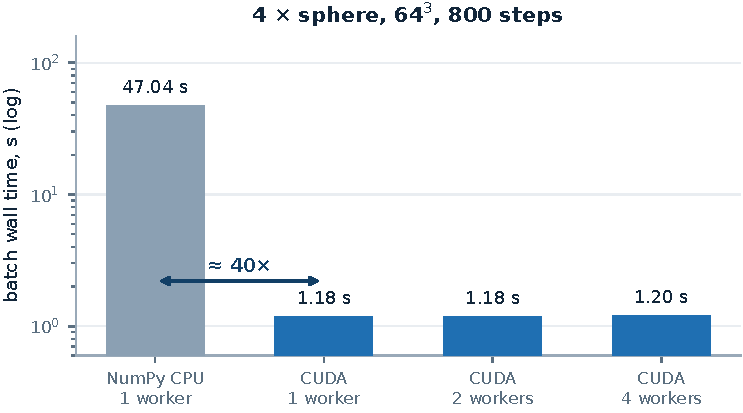
\includegraphics[width=3.4cm]{figures/chart-cpu-gpu.pdf}}

\begin{document}

{\setbeamertemplate{footline}{}
\begin{frame}[plain]
  \vspace{-2mm}
  \begin{center}
    {\Huge\bfseries\color{pwdeep} PhotonWeave}\\[4pt]
    {\large Lumerical FDTD를 대체하는 GPU 가속 FDTD 워크벤치}\\[10pt]
    {\footnotesize 브라우저 CAD + Python API + NVIDIA CUDA 네이티브 솔버\quad·\quad MIT 라이선스\quad·\quad v0.14.0.dev}\\[8pt]
    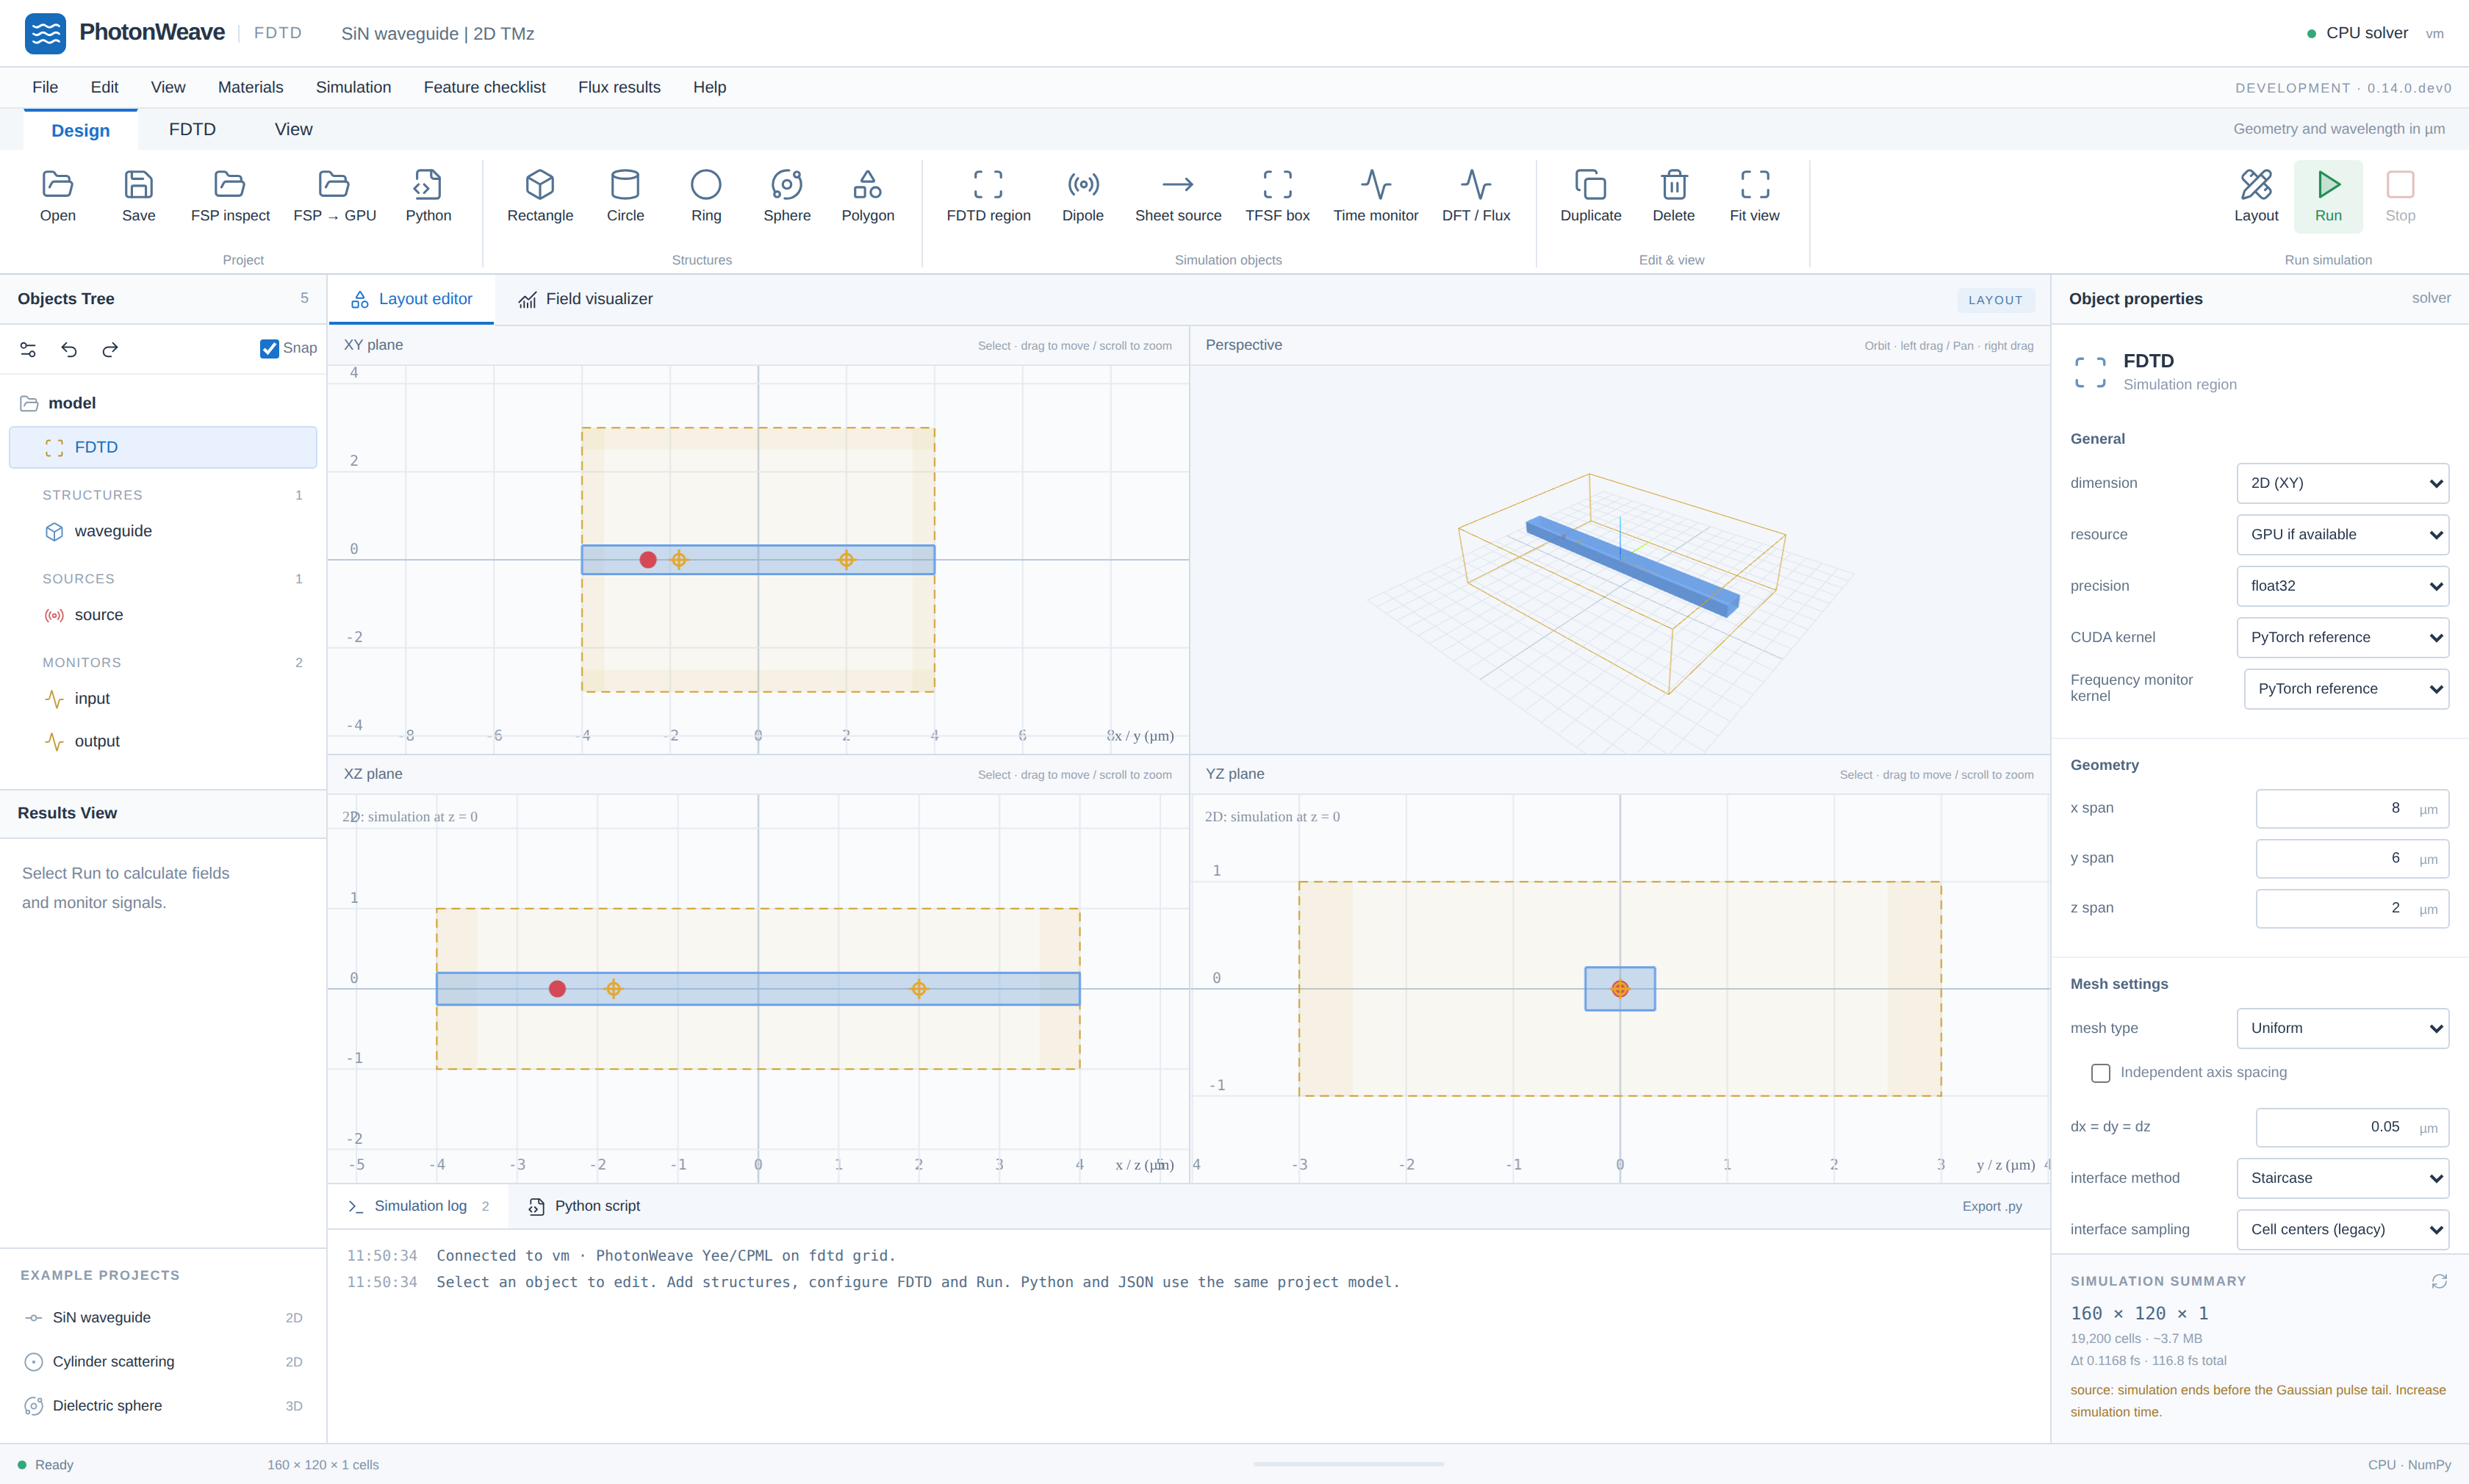
\includegraphics[width=.92\textwidth]{figures/ui-layout.png}\\[4pt]
    {\scriptsize\color{pwgrey} Hyoseok Park\quad·\quad 랩미팅 2026년 9월\quad·\quad 화면은 실제 워크벤치 캡처}
  \end{center}
\end{frame}}

\begin{frame}{오늘 이야기할 것}
  \begin{columns}[T]
    \begin{column}{.52\textwidth}
      \tableofcontents
    \end{column}
    \begin{column}{.44\textwidth}
      \begin{block}{한 줄 요약}
        상용 FDTD 워크플로를 그대로 쓰면서, 계산은 GPU에서,
        설계 루프는 Python에서 자동으로 도는 솔버를 직접 만들었습니다.
      \end{block}
      \vspace{2mm}
      \caveat{모든 속도 수치는 이 저장소에 기록된 측정값이며, 측정 조건과 한계를 슬라이드마다 같이 적었습니다.}
    \end{column}
  \end{columns}
\end{frame}

% ===========================================================================
\section{왜 직접 만들었나}
% ===========================================================================

\begin{frame}{우리 연구에서 FDTD가 병목이 되는 지점}
  \begin{columns}[T]
    \begin{column}{.46\textwidth}
      \textbf{상용 FDTD의 실제 사용 패턴}
      \begin{itemize}
        \item 구조 하나 계산 $\rightarrow$ 결과 확인 $\rightarrow$ 파라미터 수정 $\rightarrow$ 재계산
        \item 스윕/역설계는 \hl{케이스 수만큼 순차 실행}
        \item 동시 실행 개수가 보유 라이선스에 묶임
        \item 우리가 비교 기록을 가진 구성은 \hl{CPU 16 스레드 엔진} (상용 GPU 엔진은 미비교)
        \item 목적함수의 기울기(gradient)를 사용자 코드에서 받을 수 없음
      \end{itemize}
    \end{column}
    \begin{column}{.5\textwidth}
      \begin{tikzpicture}[font=\scriptsize,
        box/.style={draw=pwgrey, fill=white, rounded corners=2pt, inner sep=4pt,
                    text width=2.1cm, align=center, minimum height=9mm},
        hot/.style={box, draw=pwred, fill=pwred!8}]
        \node[box] (a) at (0,2.1) {구조 편집 (GUI)};
        \node[box] (b) at (3.1,2.1) {메시 + 실행\\(CPU 엔진)};
        \node[hot] (c) at (3.1,0.5) {대기\\수 분 $\sim$ 수 시간};
        \node[hot] (d) at (0,0.5) {사람이 다음\\파라미터 결정};
        \draw[-Stealth, pwdeep] (a)--(b);
        \draw[-Stealth, pwdeep] (b)--(c);
        \draw[-Stealth, pwdeep] (c)--(d);
        \draw[-Stealth, pwdeep] (d)--(a);
        \node[text width=4.6cm, align=center, color=pwred] at (1.55,-0.85)
          {루프 한 바퀴가 느리면\\설계 공간을 탐색할 수 없음};
      \end{tikzpicture}
    \end{column}
  \end{columns}
\end{frame}

\begin{frame}{그래서 무엇을 바꿨나}
  \vspace{-3mm}
  \begin{center}
    \begin{tikzpicture}[font=\scriptsize, scale=.76, every node/.style={transform shape},
      lay/.style={draw=pwgrey, fill=white, rounded corners=2pt, inner sep=4pt, text width=2.2cm, align=center, minimum height=8mm},
      new/.style={lay, draw=pwblue, fill=pwblue!8},
      lbl/.style={font=\scriptsize\bfseries, color=pwdeep}]

      \node[lbl, align=right] at (-.9,1.15) {기존};
      \node[lay] (a1) at (1.5,1.15) {GUI 구조 편집};
      \node[lay] (a2) at (4.3,1.15) {CPU 엔진\\1 케이스};
      \node[lay] (a3) at (7.1,1.15) {결과 파일};
      \node[lay] (a4) at (9.9,1.15) {사람이 판단};
      \draw[-Stealth, pwgrey] (a1)--(a2); \draw[-Stealth, pwgrey] (a2)--(a3); \draw[-Stealth, pwgrey] (a3)--(a4);
      \draw[-Stealth, pwgrey] (a4.north) to[out=90,in=90,looseness=.32] node[above, font=\tiny, color=pwgrey] {한 번에 한 구조} (a1.north);

      \node[lbl, align=right] at (-.9,-1.5) {PhotonWeave};
      \node[new] (b1) at (1.5,-1.5) {브라우저 CAD\\Python · FSP};
      \node[new] (b2) at (4.3,-1.5) {CUDA 네이티브\\$N$ 케이스 동시};
      \node[new] (b3) at (7.1,-1.5) {목적함수\\+ 기울기};
      \node[new] (b4) at (9.9,-1.5) {최적화기가\\자동 판단};
      \draw[-Stealth, pwblue] (b1)--(b2); \draw[-Stealth, pwblue] (b2)--(b3); \draw[-Stealth, pwblue] (b3)--(b4);
      \draw[-Stealth, pwblue] (b4.south) to[out=-90,in=-90,looseness=.32] node[below, font=\tiny, color=pwblue] {한 번에 설계 공간 전체} (b1.south);
    \end{tikzpicture}
  \end{center}
  \vspace{-2mm}
  \begin{columns}[T]
    \begin{column}{.32\textwidth}\card{2.9cm}{익숙한 UI}{Objects Tree, CAD 4뷰, Layout/Analysis 모드}\end{column}
    \begin{column}{.32\textwidth}\card{2.9cm}{GPU 네이티브}{Yee/CPML fused CUDA 커널 + CUDA Graph}\end{column}
    \begin{column}{.32\textwidth}\card{2.9cm}{미분 가능}{discrete adjoint로 $\partial f/\partial \varepsilon$ 직접 계산}\end{column}
  \end{columns}
\end{frame}

\begin{frame}{핵심 수치 한 장 요약}
  \begin{columns}[T]
    \begin{column}{.33\textwidth}
      \card{3.3cm}{6.5 -- 15.2$\times$}{Lumerical CPU(16 threads) 대비 기록된 wall time 비 \\ \textcolor{pwred}{과거 빌드 · 동일정확도 아님}}
      \vspace{3mm}
      \card{3.3cm}{9.6 -- 17.1$\times$}{동일 격자·소스·모니터에서 오픈소스 GPU 기준선 대비}
    \end{column}
    \begin{column}{.33\textwidth}
      \card{3.3cm}{$\approx$ 40$\times$}{같은 4케이스 배치: NumPy CPU 47.04 s $\rightarrow$ CUDA 1.175 s}
      \vspace{3mm}
      \card{3.3cm}{46.7 / 85.9$\times$}{adjoint 기울기 1회: CPU 대비 GPU resident (FP32 / complex FP64)}
    \end{column}
    \begin{column}{.33\textwidth}
      \card{3.3cm}{54 GiB}{48 GB VRAM을 넘는 상태를 streaming으로 전진+역전파 완료}
      \vspace{3mm}
      \card{3.3cm}{4.4e-6}{박막 해석해 대비 $R+T-1$ 잔차 (오늘 CPU에서 재현)}
    \end{column}
  \end{columns}
  \vspace{3mm}
  \caveat{각 수치의 측정 조건·베이스라인·남은 검증 항목은 해당 슬라이드에서 그대로 밝힙니다.}
\end{frame}

% ===========================================================================
\section{워크벤치: 무엇을 만들었나}
% ===========================================================================

\begin{frame}{시스템 구조}
  \begin{center}
    \begin{tikzpicture}[font=\scriptsize, scale=.88, every node/.style={transform shape},
      blk/.style={draw=pwgrey, fill=white, rounded corners=2pt, inner sep=5pt, align=center},
      hi/.style={blk, draw=pwblue, fill=pwblue!8},
      gpu/.style={blk, draw=pwgreen, fill=pwgreen!8}]

      \node[hi, text width=3.1cm] (ui) at (0,2.8) {\textbf{브라우저 워크벤치}\\Objects Tree · CAD 4뷰\\재료/메시/모니터 편집};
      \node[hi, text width=3.1cm] (py) at (4.2,2.8) {\textbf{Python API}\\\texttt{Project / Simulation}\\\texttt{BatchRunner / optimize}};
      \node[hi, text width=3.1cm] (fsp) at (8.4,2.8) {\textbf{FSP 브리지}\\독립 리더/라이터\\(.fsp 구조·설정 일부)};

      \node[blk, text width=11.2cm] (model) at (4.2,1.5) {\textbf{공통 프로젝트 모델} (JSON schema, µm 단위) — 구조 · 재료 · 소스 · 모니터 · 메시 · 경계};

      \node[blk, text width=11.2cm] (solver) at (4.2,0.3) {\textbf{솔버 코어} — Yee 업데이트 · 6면 CPML · 주기/Bloch · graded/rectilinear 메시 · ADE 분산재료};

      \node[gpu, text width=3.4cm] (torch) at (-0.1,-1.1) {PyTorch 경로\\CPU / CUDA, float32/64};
      \node[gpu, text width=3.4cm] (fused) at (4.2,-1.1) {fused CUDA 커널\\+ CUDA Graph};
      \node[gpu, text width=3.4cm] (adj) at (8.5,-1.1) {discrete adjoint\\+ checkpoint replay};

      \node[blk, text width=11.2cm, draw=pwamber, fill=pwamber!8] (mem) at (4.2,-2.3) {\textbf{메모리 계층} — VRAM resident / DRAM 스트리밍 / 파일 백킹 (space-time tile)};

      \draw[-Stealth, pwdeep] (ui)--(model); \draw[-Stealth, pwdeep] (py)--(model); \draw[-Stealth, pwdeep] (fsp)--(model);
      \draw[-Stealth, pwdeep] (model)--(solver);
      \draw[-Stealth, pwdeep] (solver)--(torch); \draw[-Stealth, pwdeep] (solver)--(fused); \draw[-Stealth, pwdeep] (solver)--(adj);
      \draw[-Stealth, pwdeep] (torch)--(mem); \draw[-Stealth, pwdeep] (fused)--(mem); \draw[-Stealth, pwdeep] (adj)--(mem);
    \end{tikzpicture}
  \end{center}
  \vspace{1mm}
  \caveat{그리드/백엔드 기반은 오픈소스 flaport/fdtd(MIT)를 사용하고, Yee 미분·CPML·주기/Bloch·CUDA Graph 실행은 직접 구현했습니다.}
\end{frame}

\begin{frame}{익숙한 화면 그대로: Layout 모드}
  \begin{center}
    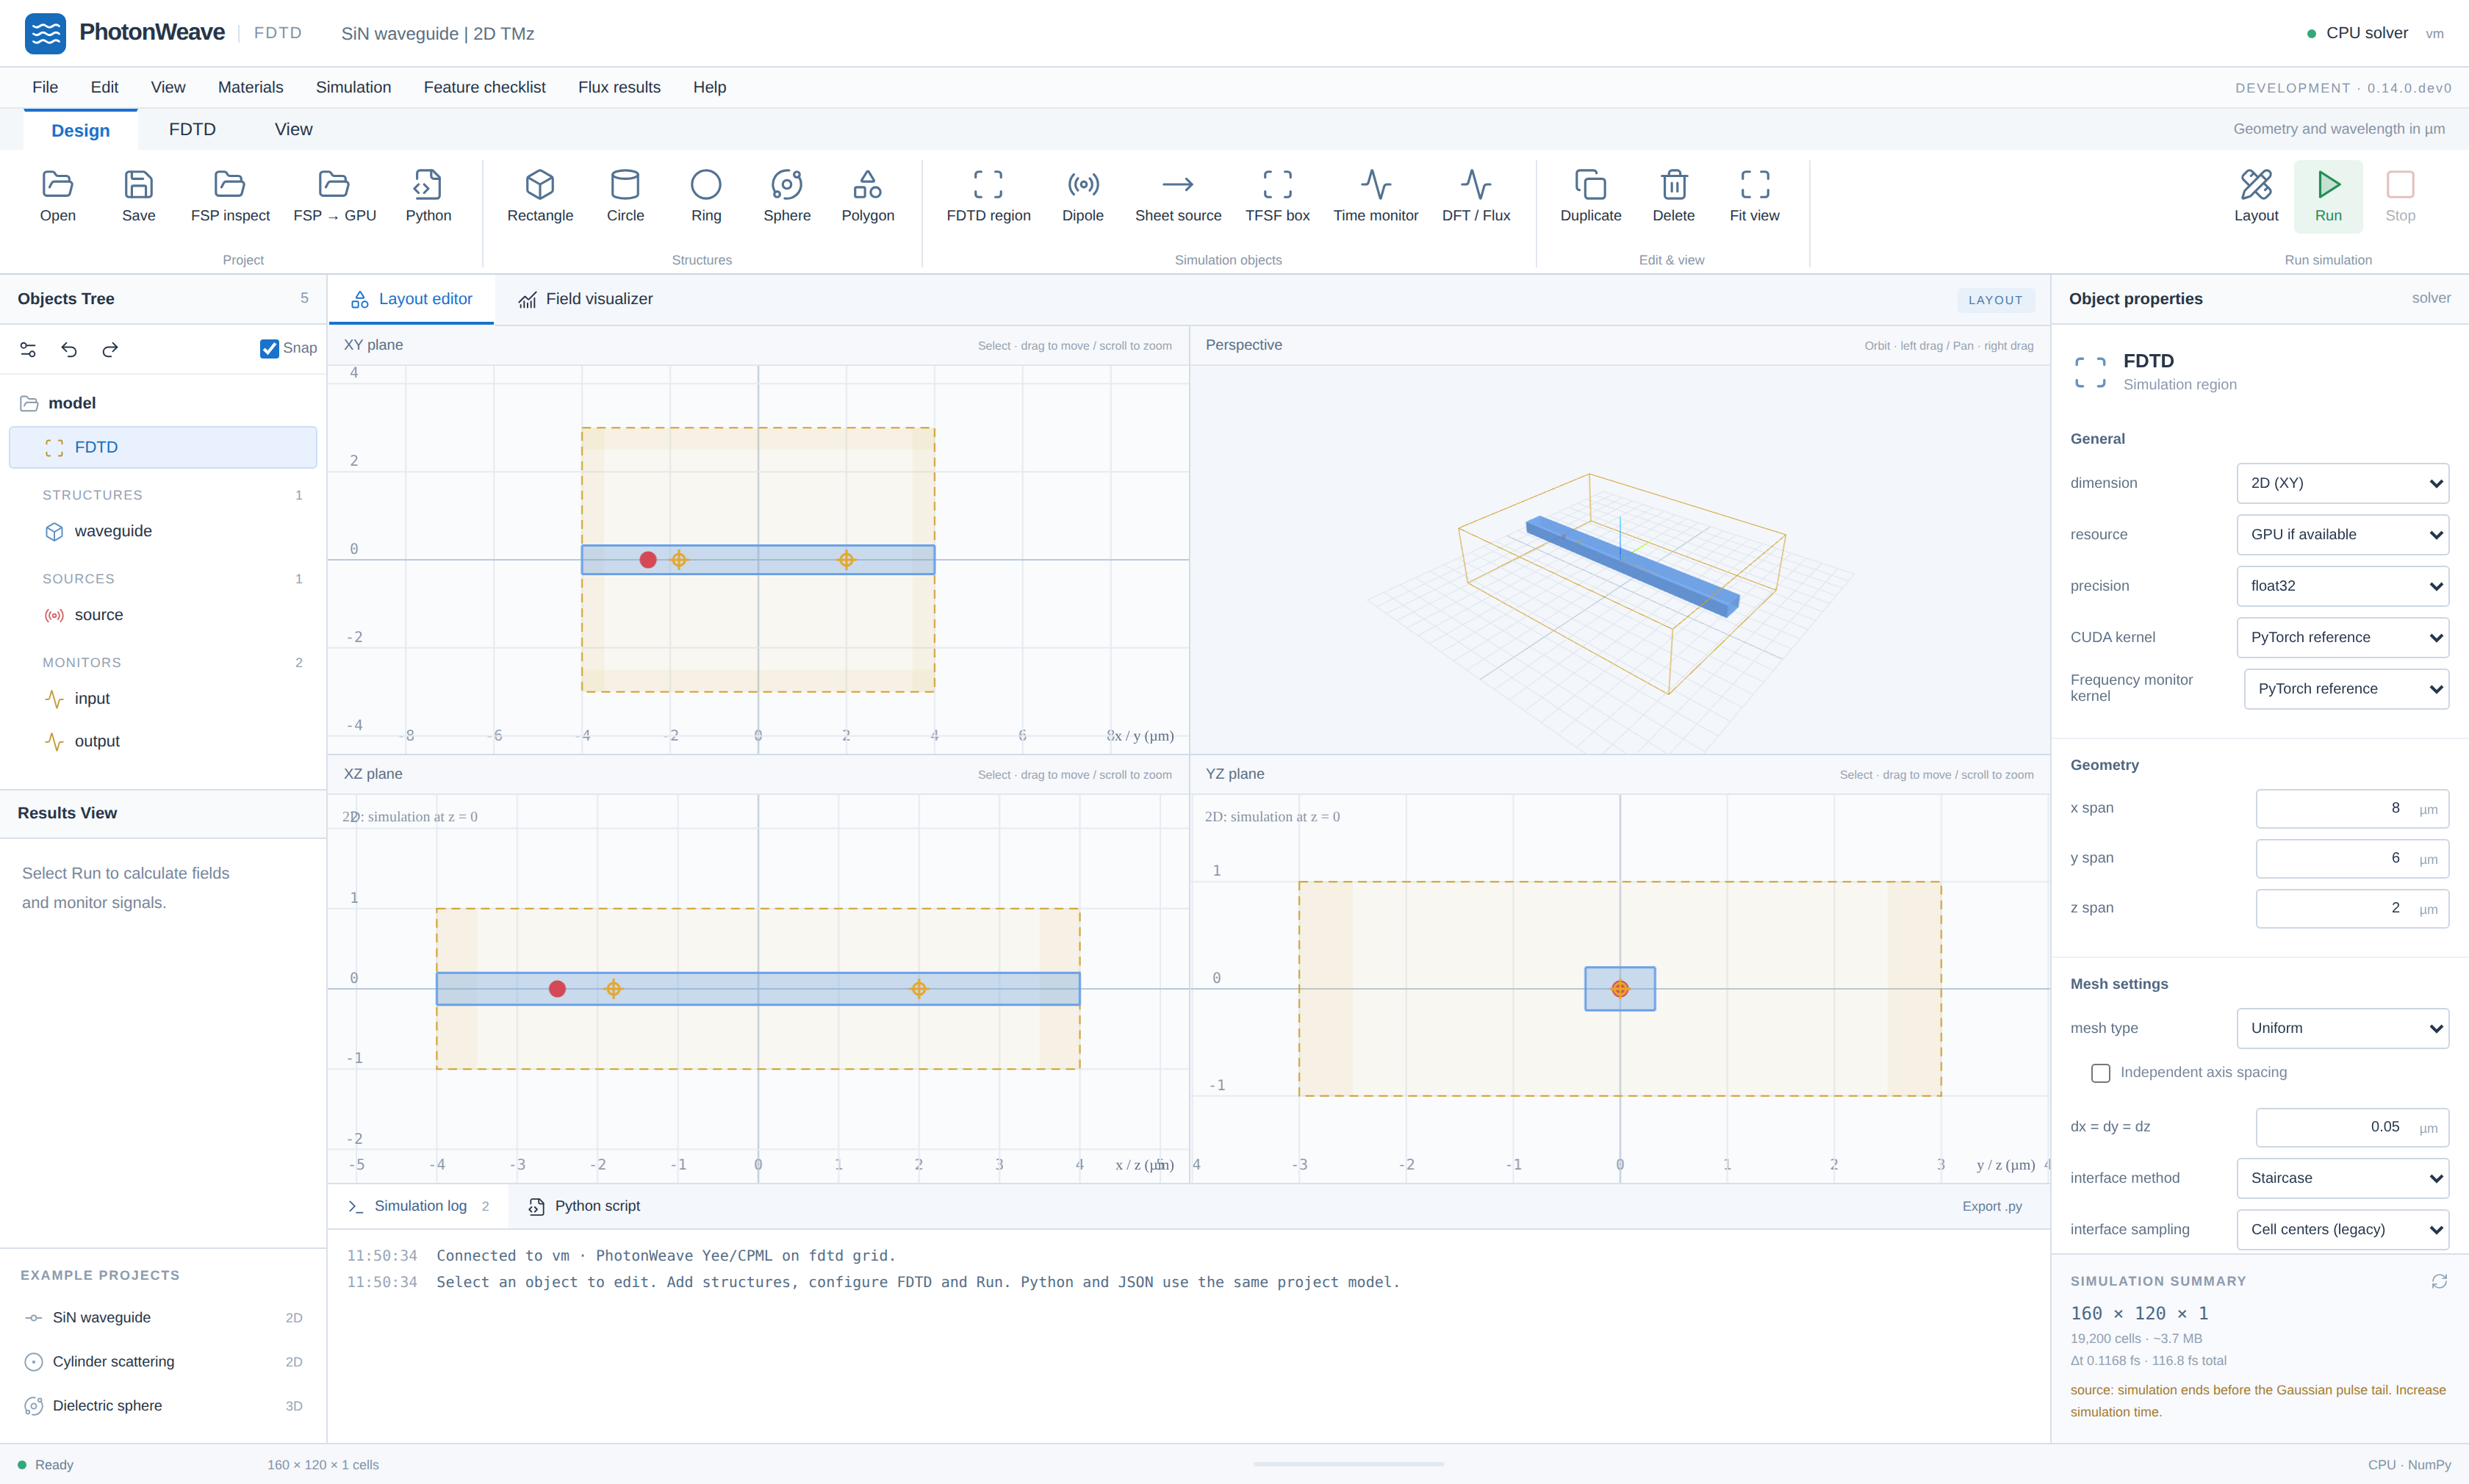
\includegraphics[width=.93\textwidth]{figures/ui-layout.png}\\[1mm]
    \caveat{Objects Tree · XY/XZ/YZ + Perspective · Object properties · 재료/메시 설정 · Python export 까지 상용 FDTD와 같은 순서로 작업합니다.}
  \end{center}
\end{frame}

\begin{frame}{계산이 끝나면 그대로 Analysis 모드}
  \begin{center}
    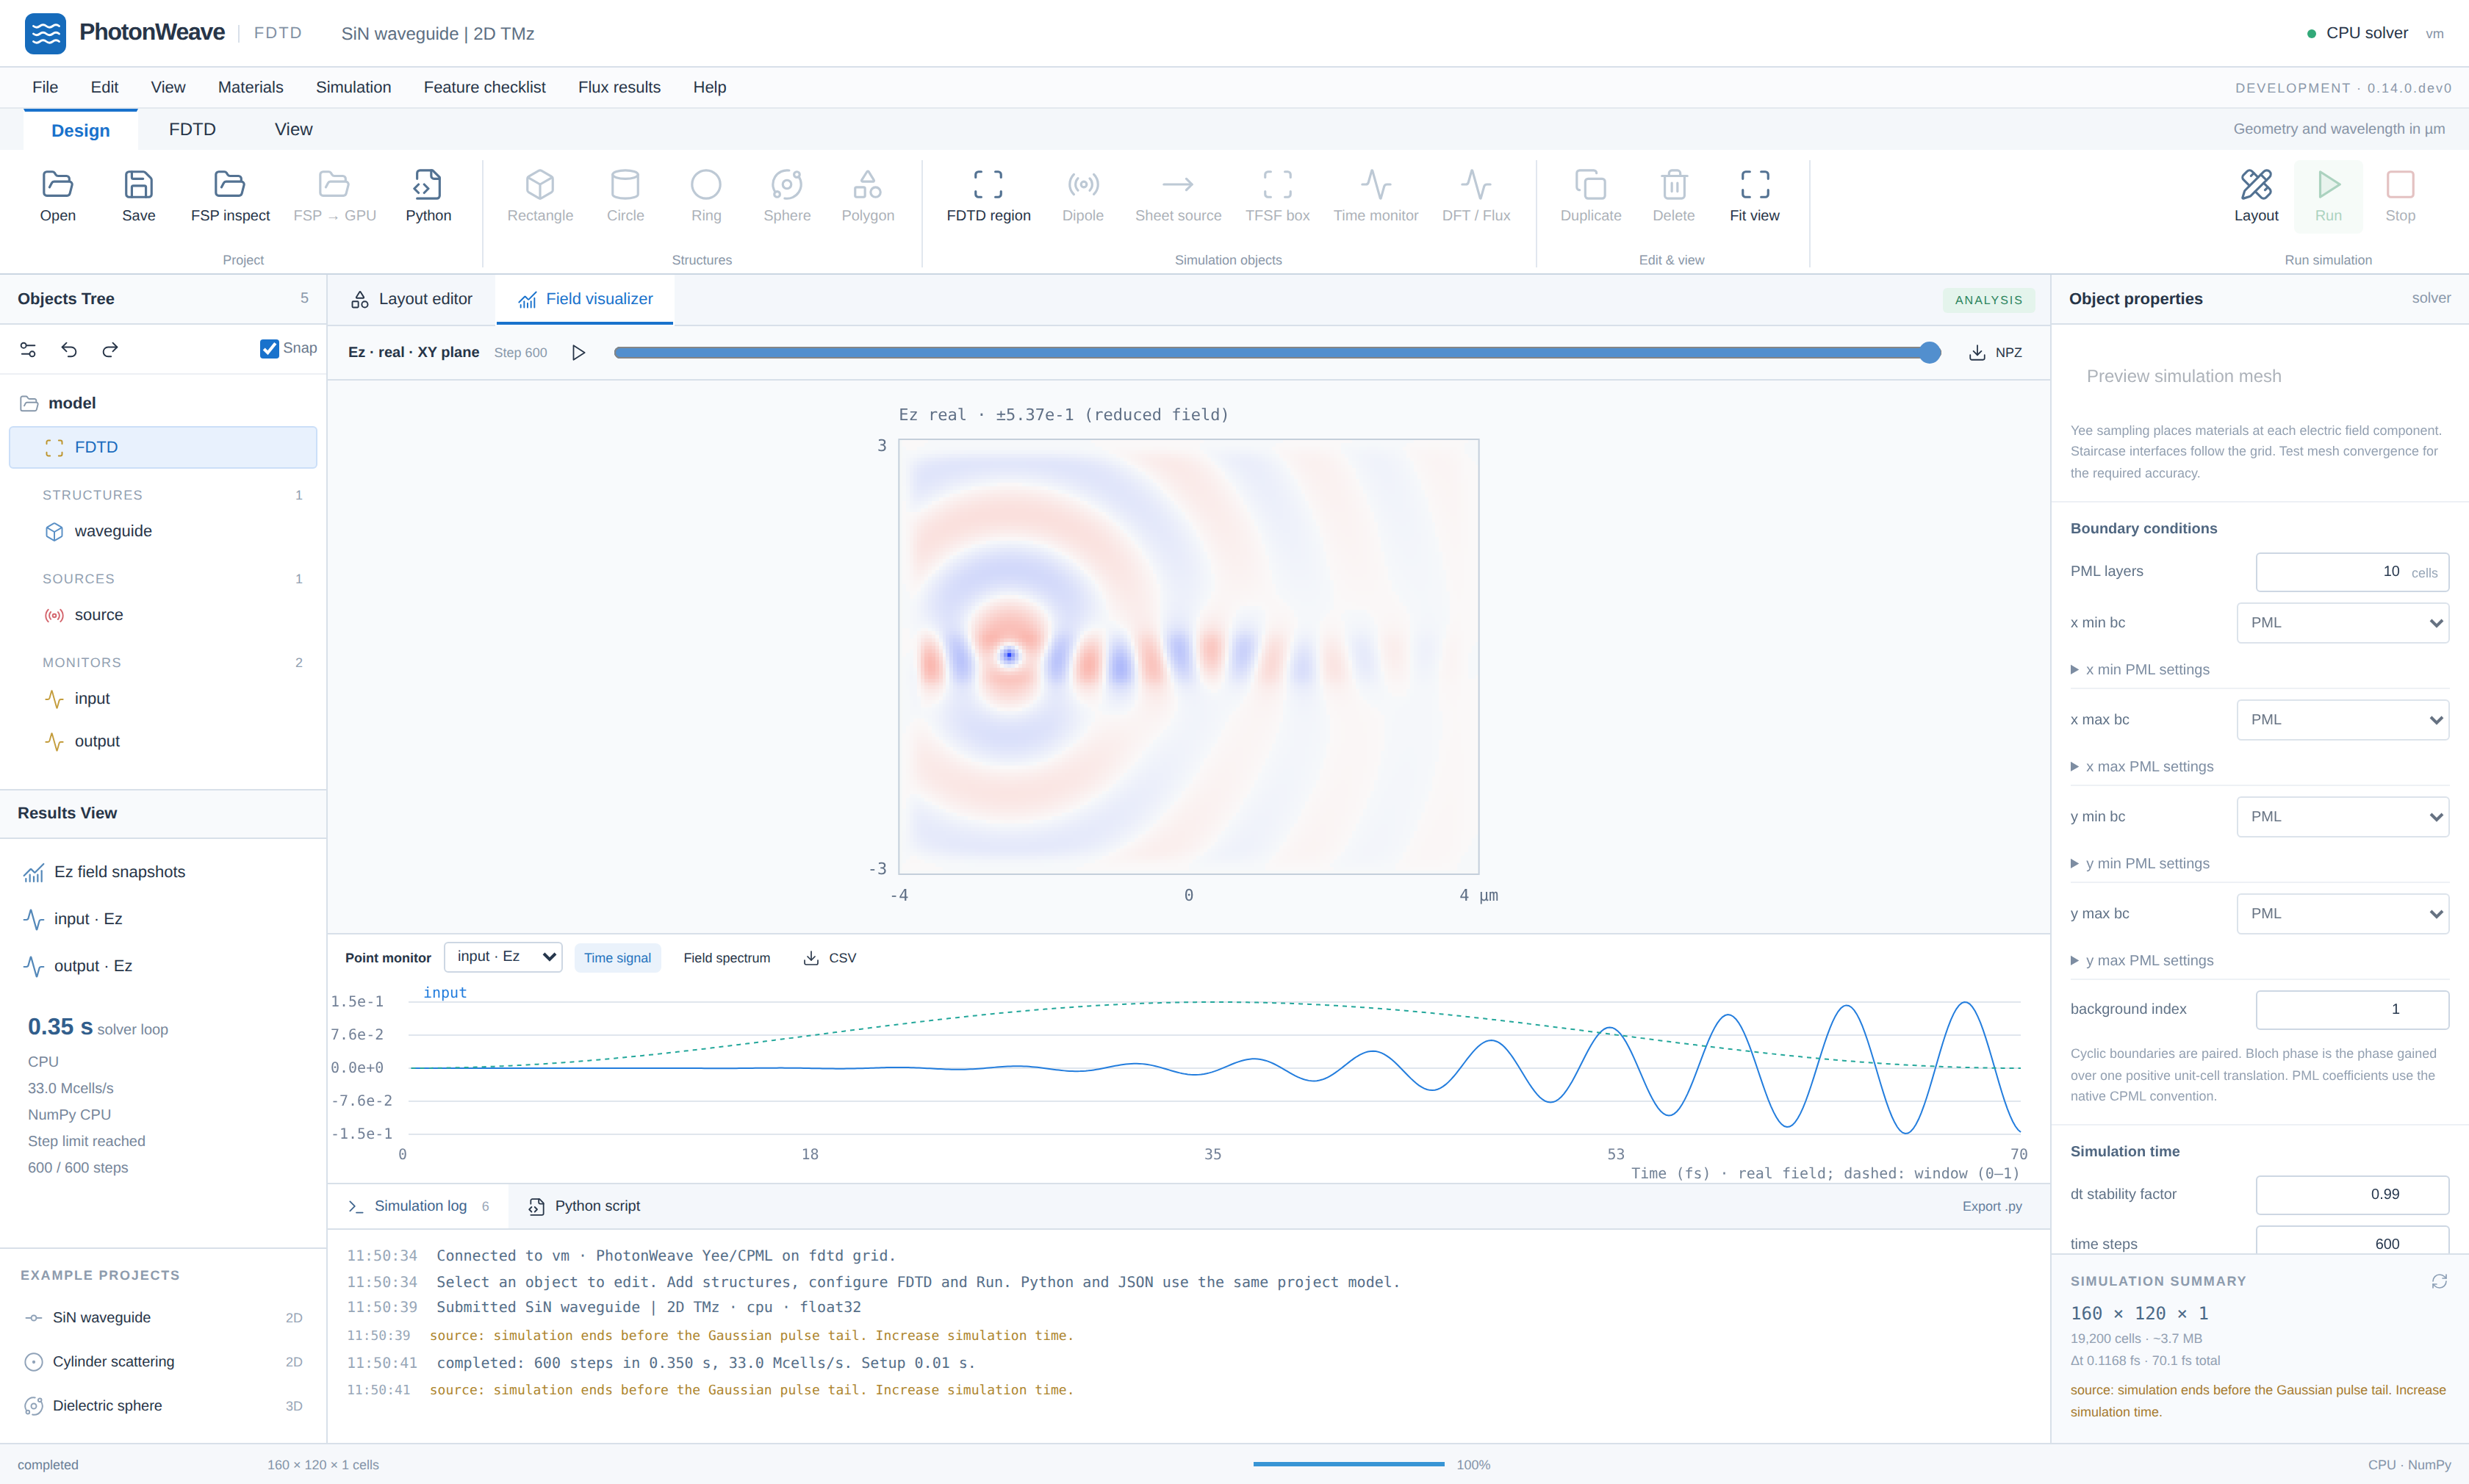
\includegraphics[width=.93\textwidth]{figures/ui-results.png}\\[1mm]
    \caveat{필드 스냅샷 애니메이션 · 포인트 모니터 시계열/스펙트럼 · NPZ/CSV 내보내기. 실행 중 레이아웃 잠금도 동일합니다.}
  \end{center}
\end{frame}

\begin{frame}[fragile]{같은 프로젝트를 세 가지 입구에서}
  \begin{columns}[T]
    \begin{column}{.48\textwidth}
      \begin{center}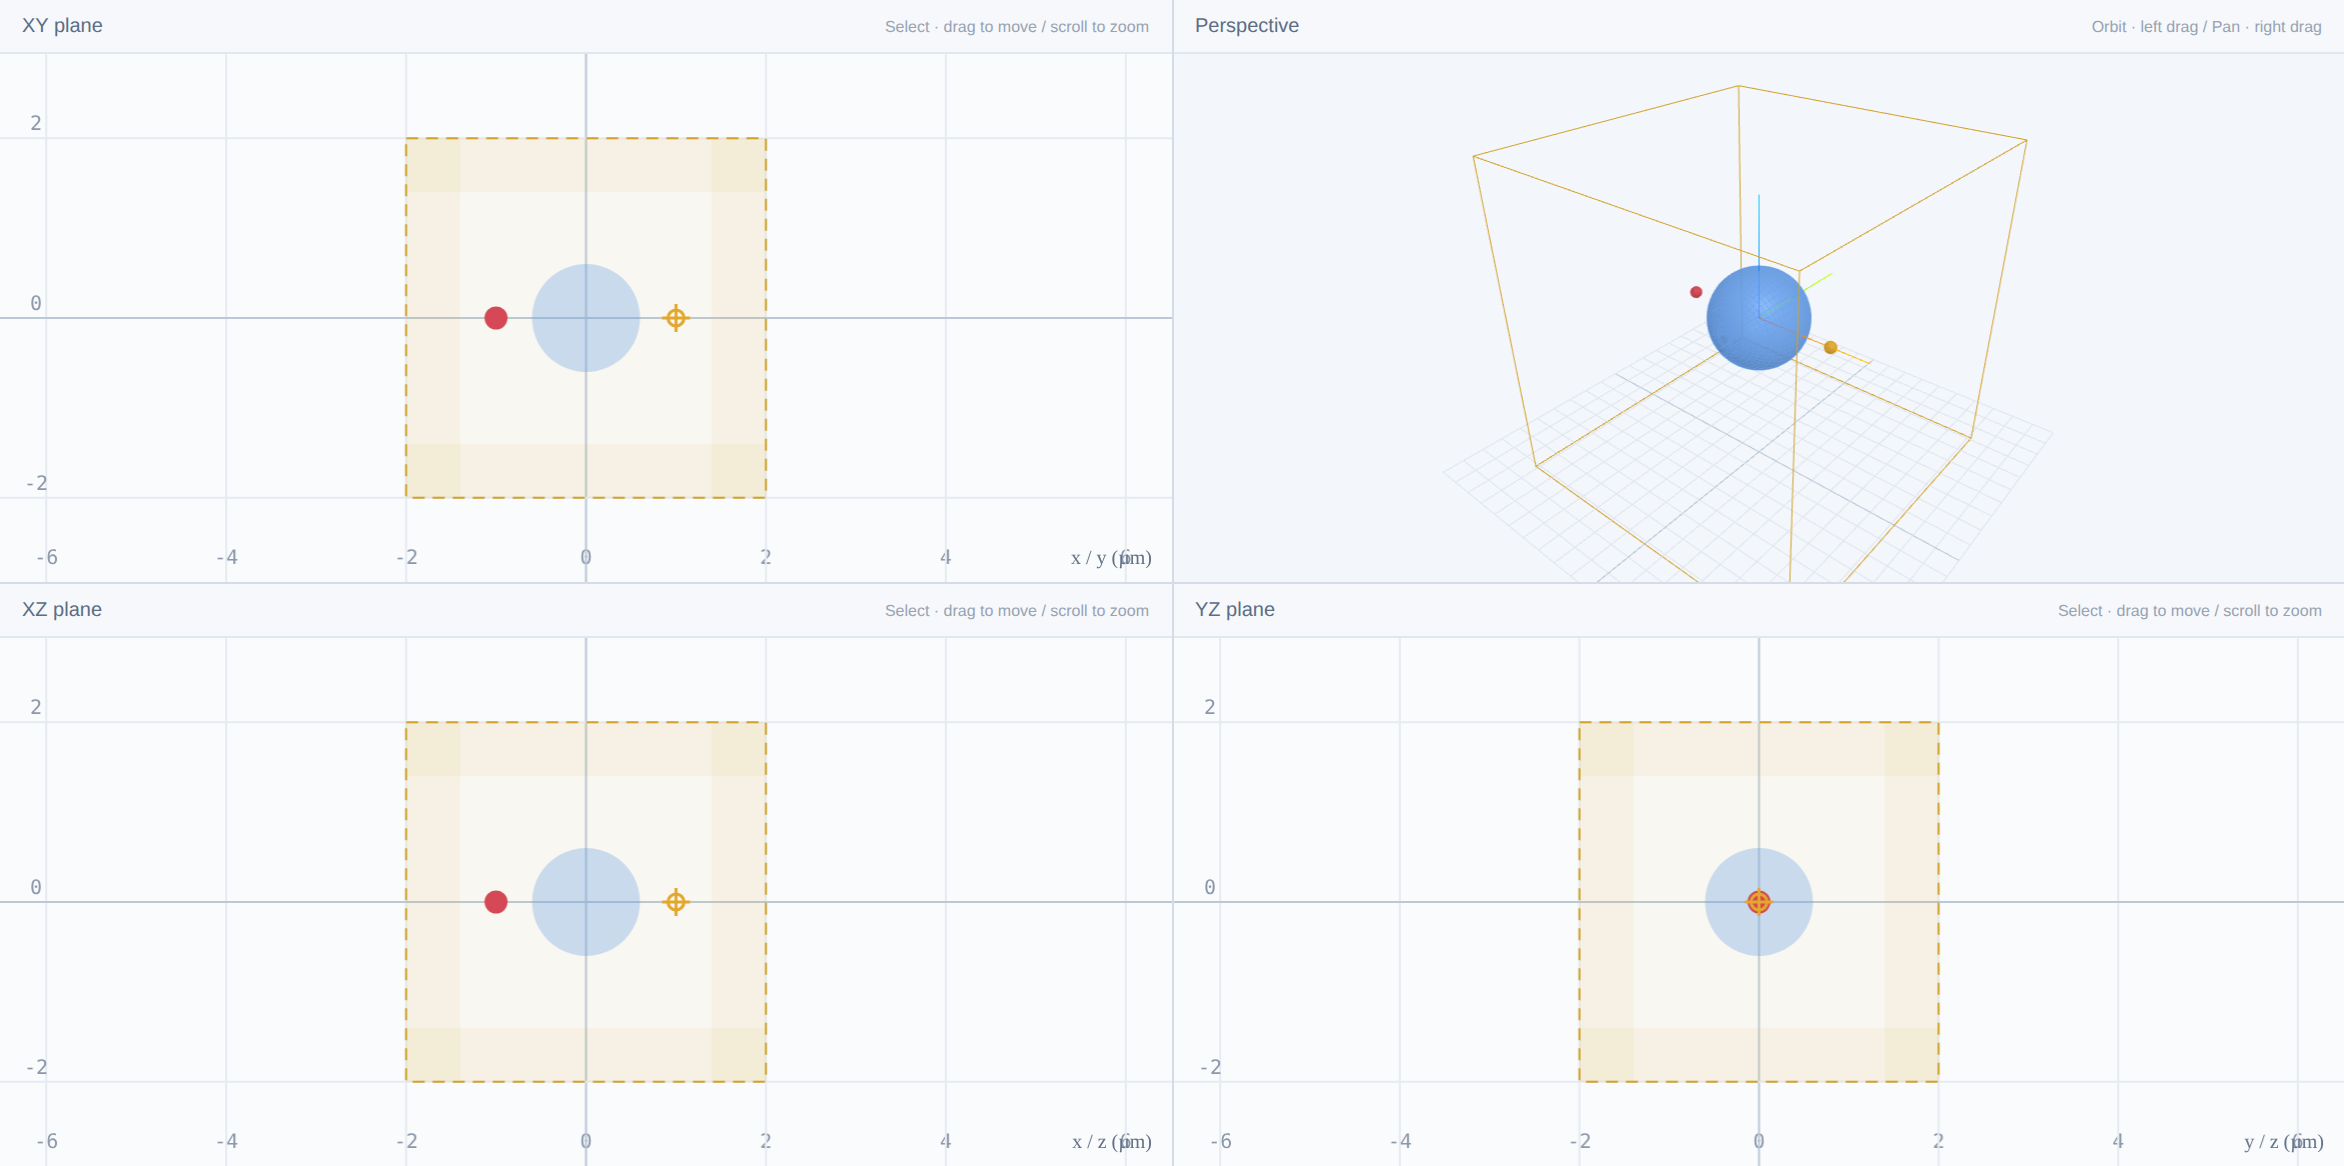
\includegraphics[width=\textwidth]{figures/ui-sphere-viewports.png}\end{center}
      \caveat{3D 예제(유전체 구)의 4뷰 CAD. 브라우저에서 만든 구조가 그대로 Python 객체입니다.}
    \end{column}
    \begin{column}{.48\textwidth}
\begin{lstlisting}[basicstyle=\ttfamily\tiny]
from photonweave import (Project, Region,
    Structure, Source, Monitor, Simulation)

project = Project(
  name="My waveguide",
  region=Region(size=(8, 6, 2), mesh=0.05,
                steps=1000, backend="cuda"),
  structures=[Structure(name="core",
                        size=(8, 0.65, 0.4))],
  sources=[Source(center=(-2.5, 0, 0),
                  wavelength=1.55)],
  monitors=[Monitor(name="output",
                    center=(2, 0, 0))])

result = Simulation(project).run()
result.save("results/run.npz")
\end{lstlisting}
      \vspace{1mm}
      \caveat{UI $\rightarrow$ JSON $\rightarrow$ Python이 같은 모델. UI의 \texttt{Export .py}가 실행 가능한 스크립트를 그대로 만들어 줍니다.}
    \end{column}
  \end{columns}
\end{frame}

% ===========================================================================
\section{엔진 내부}
% ===========================================================================

\begin{frame}{Yee 격자와 leapfrog 시간 전개}
  \begin{columns}[T]
    \begin{column}{.5\textwidth}
      \begin{center}
        \begin{tikzpicture}[x={(1.25cm,0cm)}, y={(0cm,1.25cm)}, z={(-0.62cm,-0.47cm)},
                            font=\scriptsize, line join=round]
          \foreach \dx in {0, 2.35} {
            \begin{scope}[xshift=\dx cm]
              \draw[pwgrey!75] (0,0,0)--(1,0,0)--(1,1,0)--(0,1,0)--cycle;
              \draw[pwgrey!35] (0,0,1)--(1,0,1)--(1,1,1)--(0,1,1)--cycle;
              \draw[pwgrey!35] (0,0,0)--(0,0,1); \draw[pwgrey!35] (1,0,0)--(1,0,1);
              \draw[pwgrey!35] (1,1,0)--(1,1,1); \draw[pwgrey!35] (0,1,0)--(0,1,1);
            \end{scope}}
          % (1) E lives on cell edges
          \draw[-Stealth, pwblue, very thick] (0,0,0)--(.7,0,0);
          \node[pwblue, anchor=north] at (.5,0,0) {$E_x$};
          \draw[-Stealth, pwblue, very thick] (0,0,0)--(0,.7,0);
          \node[pwblue, anchor=east] at (0,.55,0) {$E_y$};
          \draw[-Stealth, pwblue, very thick] (0,0,0)--(0,0,.7);
          \node[pwblue, anchor=south east] at (0,0,.6) {$E_z$};
          \fill[pwdeep] (0,0,0) circle (1.1pt);
          \node[anchor=north, font=\scriptsize] at (.5,-.34,0) {$\mathbf{E}$: 모서리};
          % (2) H lives on face centres
          \begin{scope}[xshift=2.55cm]
            % each component sits at its own face centre and points along its axis
            \draw[-Stealth, pwred, very thick] (1,.5,.5)--(1.5,.5,.5);
            \node[pwred, anchor=west] at (1.5,.5,.5) {$H_x$};
            \draw[-Stealth, pwred, very thick] (.5,1,.5)--(.5,1.45,.5);
            \node[pwred, anchor=south] at (.5,1.45,.5) {$H_y$};
            \draw[-Stealth, pwred, very thick] (.5,.5,1)--(.5,.5,1.5);
            \node[pwred, anchor=east] at (.5,.5,1.5) {$H_z$};
            \fill[pwred!70] (1,.5,.5) circle (1.1pt);
            \fill[pwred!70] (.5,1,.5) circle (1.1pt);
            \fill[pwred!70] (.5,.5,1) circle (1.1pt);
            \node[anchor=north, font=\scriptsize] at (.5,-.34,0) {$\mathbf{H}$: 면 중심};
          \end{scope}
        \end{tikzpicture}
      \end{center}
      \vspace{1mm}
      {\footnotesize
      \[\varepsilon\frac{\partial \mathbf{E}}{\partial t}=\nabla\times\mathbf{H},\qquad
        \mu\frac{\partial \mathbf{H}}{\partial t}=-\nabla\times\mathbf{E}\]}
      \caveat{E는 모서리, H는 면 중심. 2차 정확도 중심차분, CFL 안정계수 기본 0.99.}
    \end{column}
    \begin{column}{.48\textwidth}
      \begin{center}
        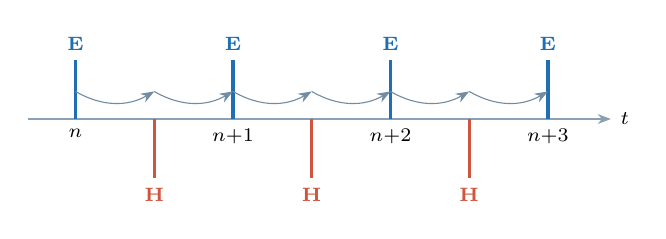
\begin{tikzpicture}[font=\scriptsize]
          \draw[-Stealth, pwgrey] (0,0)--(7.4,0) node[right, black] {$t$};
          \foreach \x/\l in {0.6/{$n$}, 2.6/{$n{+}1$}, 4.6/{$n{+}2$}, 6.6/{$n{+}3$}} {
            \draw[pwblue, very thick] (\x,0)--(\x,.75);
            \node[pwblue, above] at (\x,.75) {$\mathbf{E}$};
            \node[below, black] at (\x,0) {\l};}
          \foreach \x in {1.6, 3.6, 5.6} {
            \draw[pwred, very thick] (\x,0)--(\x,-.75);
            \node[pwred, below] at (\x,-.75) {$\mathbf{H}$};}
          \foreach \a/\b in {0.6/1.6, 1.6/2.6, 2.6/3.6, 3.6/4.6, 4.6/5.6, 5.6/6.6}
            \draw[-Stealth, pwdeep!60] (\a,.35) to[out=-30,in=210] (\b,.35);
        \end{tikzpicture}
      \end{center}
      \vspace{2mm}
      \begin{itemize}\footnotesize
        \item 3D 6성분 + 2D(z-불변) TMz/TEz
        \item float32 / float64, 실수장과 복소장(Bloch) 모두
        \item 자기장 소스는 H half-step 시각에 주입
        \item CUDA Graph로 스텝 커널 launch 오버헤드 제거
      \end{itemize}
    \end{column}
  \end{columns}
\end{frame}

\begin{frame}{경계 조건: 6면 CPML과 주기/Bloch}
  \begin{columns}[T]
    \begin{column}{.52\textwidth}
      \begin{center}
        \begin{tikzpicture}[font=\scriptsize]
          \fill[pwamber!18] (0,0) rectangle (6.2,4.2);
          \fill[white] (.75,.95) rectangle (5.45,3.45);
          \draw[pwamber, dashed] (0,0) rectangle (6.2,4.2);
          \draw[pwgrey] (.75,.95) rectangle (5.45,3.45);
          \node[pwamber!80!black] at (3.1,3.85) {CPML (면마다 두께·$\sigma$·$\kappa$·$\alpha$ 독립)};
          % structure
          \fill[pwsky!50, draw=pwdeep] (2.3,1.8) rectangle (3.9,2.6);
          \node at (3.1,2.2) {구조};
          % source
          \draw[pwred, very thick] (1.3,1.2)--(1.3,3.2);
          \node[pwred, rotate=90, anchor=south] at (1.15,2.2) {source};
          % monitor
          \draw[pwgreen, very thick, dashed] (4.7,1.2)--(4.7,3.2);
          \node[pwgreen, rotate=90, anchor=north] at (4.9,2.2) {monitor};
          % periodic / Bloch pair
          \draw[-Stealth, pwblue] (.9,.62)--(5.3,.62);
          \node[pwblue, below] at (3.1,.62) {주기 / Bloch 쌍\quad $e^{i\mathbf{k}\cdot\mathbf{a}}$};
        \end{tikzpicture}
      \end{center}
    \end{column}
    \begin{column}{.44\textwidth}
      \begin{itemize}\footnotesize
        \item \hl{Convolutional PML}: 3D 6면 / 2D 4면, 면별 레이어 수와 다항식 차수 독립 설정
        \item \hl{Periodic / Bloch} 쌍: 복소 E/H를 유지하고, sheet 소스가 지정 Bloch 위상을 자동 적용
        \item Bloch 스냅샷은 real / imag / magnitude / phase 선택, NPZ는 완전한 복소 데이터 보존
        \item \textcolor{pwred}{아직 없음}: 대칭/반대칭 경계, PEC/PMC
      \end{itemize}
      \vspace{1mm}
      \caveat{경계 규약과 검증은 docs/BOUNDARIES.md에 정리되어 있습니다.}
    \end{column}
  \end{columns}
\end{frame}

\begin{frame}{소스: 점 · 면 · 단방향 · TFSF}
  \begin{center}
    \begin{tikzpicture}[font=\tiny, node distance=2mm]
      \foreach \i/\name in {0/{점 dipole (E/H)}, 1/{soft sheet (양방향)}, 2/{one-way 주기 평면}, 3/{closed TFSF box}} {
        \begin{scope}[xshift=\i*3.25cm]
          \draw[pwgrey] (0,0) rectangle (2.9,2.3);
          \node[below, font=\scriptsize] at (1.45,-.1) {\name};
        \end{scope}}
      % dipole
      \fill[pwred] (0.9,1.15) circle (2pt);
      \foreach \r in {.35,.6,.85} \draw[pwsky] (0.9,1.15) circle (\r);
      % soft sheet
      \draw[pwred, very thick] (4.3,.45)--(4.3,1.95);
      \draw[-Stealth, pwsky] (4.4,1.5)--(5.3,1.5); \draw[-Stealth, pwsky] (4.2,1.5)--(3.4,1.5);
      \draw[-Stealth, pwsky] (4.4,.9)--(5.3,.9); \draw[-Stealth, pwsky] (4.2,.9)--(3.4,.9);
      % one-way
      \draw[pwred, very thick] (7.2,.45)--(7.2,1.95);
      \draw[-Stealth, pwblue] (7.3,1.5)--(8.6,1.5); \draw[-Stealth, pwblue] (7.3,.9)--(8.6,.9);
      \node[pwgrey] at (6.9,1.2) {0};
      % tfsf
      \draw[pwred, thick, dashed] (10.05,.6) rectangle (12.25,1.9);
      \fill[pwsky!45, draw=pwdeep] (11.15,1.25) circle (.3);
      \draw[-Stealth, pwblue] (10.2,1.62)--(10.95,1.62);
      \draw[-Stealth, pwgreen] (11.5,1.0)--(12.55,.62);
      \node[pwgreen, anchor=west, font=\tiny] at (12.35,1.0) {scattered};
    \end{tikzpicture}
  \end{center}
  \vspace{2mm}
  \begin{columns}[T]
    \begin{column}{.62\textwidth}
      \begin{itemize}\footnotesize
        \item Gaussian / 연속파 / 샘플 파형, Cartesian 또는 $\theta,\phi$ 방향
        \item 자동 파장·주파수 범위 지정(broadband), chirp, endpoint tapering
        \item one-way와 TFSF는 \hl{현재 수직 입사}만 지원 — 경사 입사와 도파로 모드 소스는 미구현
      \end{itemize}
    \end{column}
    \begin{column}{.34\textwidth}
      \caveat{TFSF는 산란 단면적을 Mie 해석해와 비교해 검증했습니다(뒤 슬라이드).}
    \end{column}
  \end{columns}
\end{frame}

\begin{frame}{메시: uniform · graded · 축별 독립(rectilinear)}
  \begin{columns}[T]
    \begin{column}{.46\textwidth}
      \begin{center}
        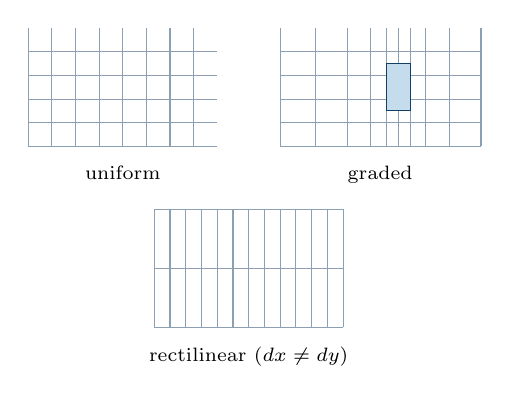
\begin{tikzpicture}[font=\tiny]
          % uniform
          \begin{scope}
            \foreach \x in {0,0.3,...,2.4} \draw[pwgrey] (\x,0)--(\x,1.5);
            \foreach \y in {0,0.3,...,1.5} \draw[pwgrey] (0,\y)--(2.4,\y);
            \node[below, font=\scriptsize] at (1.2,-.12) {uniform};
          \end{scope}
          % graded
          \begin{scope}[xshift=3.2cm]
            \foreach \x in {0,0.45,0.85,1.15,1.35,1.5,1.65,1.85,2.15,2.55} \draw[pwgrey] (\x,0)--(\x,1.5);
            \foreach \y in {0,0.3,...,1.5} \draw[pwgrey] (0,\y)--(2.55,\y);
            \fill[pwsky!40, draw=pwdeep] (1.35,.45) rectangle (1.65,1.05);
            \node[below, font=\scriptsize] at (1.27,-.12) {graded};
          \end{scope}
          % rectilinear
          \begin{scope}[yshift=-2.3cm, xshift=1.6cm]
            \foreach \x in {0,0.2,...,2.4} \draw[pwgrey] (\x,0)--(\x,1.5);
            \foreach \y in {0,0.75,1.5} \draw[pwgrey] (0,\y)--(2.4,\y);
            \node[below, font=\scriptsize] at (1.2,-.12) {rectilinear ($dx \neq dy$)};
          \end{scope}
        \end{tikzpicture}
      \end{center}
    \end{column}
    \begin{column}{.5\textwidth}
      \begin{itemize}\footnotesize
        \item 축별 독립 간격과 명시적 node 배열, 직사각형 CFL, 물리 두께 기준 PML
        \item 횡방향으로 균일한 문제(층 구조, 박막)에서는 \num{4.33--13.39$\times$} 배치 시간 감소
        \item 같은 실제 시간 스텝, 같은 관측량에서 \hl{72개 정확도 게이트 모두 통과} (최대 상대 L2 5.95e-15)
        \item 재료 경계는 기본 staircase, 실험적 subpixel 연산자 선택 가능
      \end{itemize}
      \source{README.md · Rectilinear mesh and batch ablation}
    \end{column}
  \end{columns}
\end{frame}

\begin{frame}{CUDA 실행 모델: 왜 빨라지는가}
  \begin{center}
    \begin{tikzpicture}[font=\scriptsize, scale=.92, every node/.style={transform shape},
      blk/.style={draw=pwgrey, fill=white, rounded corners=2pt, inner sep=4pt, align=center,
                  text width=2.25cm, minimum height=1.25cm}]
      % stacked grids
      \foreach \i in {0,1,2} {
        \begin{scope}[xshift=\i*0.3cm, yshift=-\i*0.26cm]
          \fill[pwsky!30, draw=pwdeep] (0,0) rectangle (1.5,1.15);
        \end{scope}}
      \node[align=center, font=\scriptsize] at (1.0,-1.15) {독립 구조 $N$개\\같은 격자 topology};

      \node[blk] (batch) at (3.9,0.3) {배치 축 E/H 텐서\\$(N, N_x, N_y, N_z)$};
      \node[blk] (kernel) at (6.6,0.3) {fused Yee/CPML\\커널 1회 launch};
      \node[blk] (graph) at (9.3,0.3) {CUDA Graph\\replay};
      \node[blk] (out) at (12.0,0.3) {공유 모니터\\DFT 커널};

      \draw[-Stealth, pwdeep] (2.3,0.3)--(batch);
      \draw[-Stealth, pwdeep] (batch)--(kernel);
      \draw[-Stealth, pwdeep] (kernel)--(graph);
      \draw[-Stealth, pwdeep] (graph)--(out);
    \end{tikzpicture}
  \end{center}
  \vspace{2mm}
  \begin{columns}[T]
    \begin{column}{.32\textwidth}
      \begin{block}{\footnotesize 커널 융합}
        \footnotesize E/H 업데이트·CPML·소스·트레이스를 한 커널로. PyTorch 참조 경로 대비 \num{3.67--5.76$\times$}
      \end{block}
    \end{column}
    \begin{column}{.32\textwidth}
      \begin{block}{\footnotesize 배치 축}
        \footnotesize 케이스별 반복 대신 한 launch. 결과는 개별 실행과 \hl{bitwise 동일}
      \end{block}
    \end{column}
    \begin{column}{.32\textwidth}
      \begin{block}{\footnotesize 모니터 공유}
        \footnotesize 평면 보간 + DFT 누적을 케이스·평면에 걸쳐 공유: \num{3.63--8.12$\times$}
      \end{block}
    \end{column}
  \end{columns}
\end{frame}

% ===========================================================================
\section{정확도 검증}
% ===========================================================================

\begin{frame}{해석해와 비교 1: 유전체 박막의 $R$, $T$}
  \begin{center}
    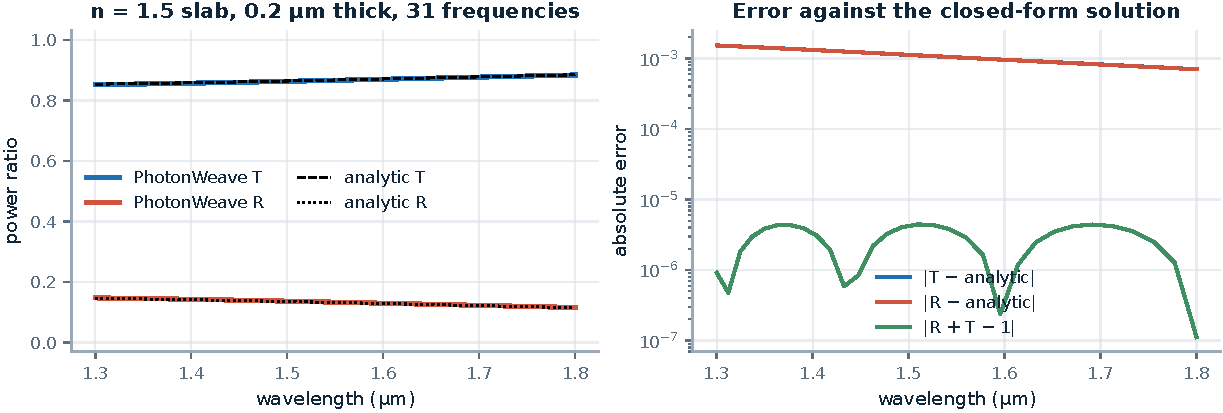
\includegraphics[width=.94\textwidth]{figures/field-slab-validation.pdf}
  \end{center}
  \vspace{-2mm}
  \begin{columns}[T]
    \begin{column}{.62\textwidth}
      \footnotesize
      동일한 공기 reference로 정규화, 반사는 복소 E/H incident subtraction.
      최대 절대 오차 $|T-T_\text{exact}| = $ \num{1.53e-3}, 에너지 잔차 $|R+T-1| = $ \num{4.44e-6}.
    \end{column}
    \begin{column}{.34\textwidth}
      \caveat{이 그림은 오늘 이 저장소에서 CPU float64로 다시 돌려 만든 결과입니다 (1.2초).}
    \end{column}
  \end{columns}
\end{frame}

\begin{frame}{해석해와 비교 2: TFSF 구 산란 vs Mie 급수}
  \begin{columns}[T]
    \begin{column}{.52\textwidth}
      \begin{center}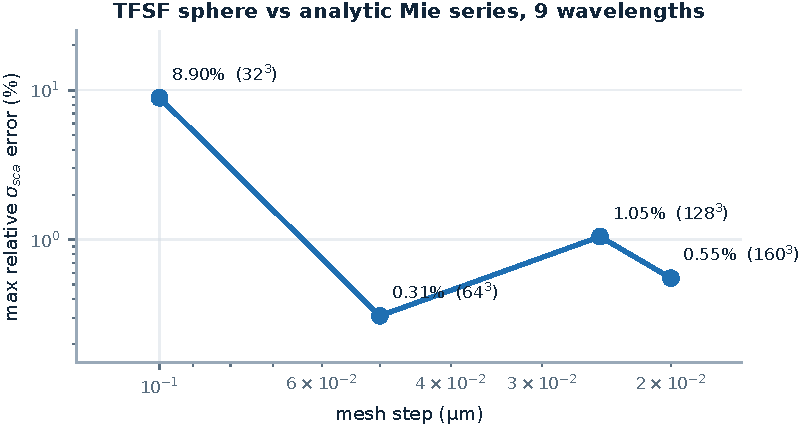
\includegraphics[width=\textwidth]{figures/chart-mie.pdf}\end{center}
    \end{column}
    \begin{column}{.44\textwidth}
      \begin{itemize}\footnotesize
        \item 반지름 0.3 µm, $n=1.5$ 구, 1.3--1.8 µm 9개 파장
        \item 도메인 크기·물리 PML 두께·120 fs 지속시간 고정
        \item 0.05 µm 메시에서 최대 오차 \num{0.31\%}
        \item \alert{오차가 단조 감소하지 않음}: 0.025 µm에서 1.05\%로 증가
        \item staircase 경계 + TFSF 보정의 상호작용으로 해석 중
      \end{itemize}
      \vspace{1mm}
      \caveat{가장 좋은 행을 정확도 보장으로 쓰지 않습니다. 정량 결과에는 수렴 테스트가 필요합니다.}
    \end{column}
  \end{columns}
\end{frame}

\begin{frame}{우리 연구 대상으로 직접 계산 1: photonic band gap}
  \begin{center}
    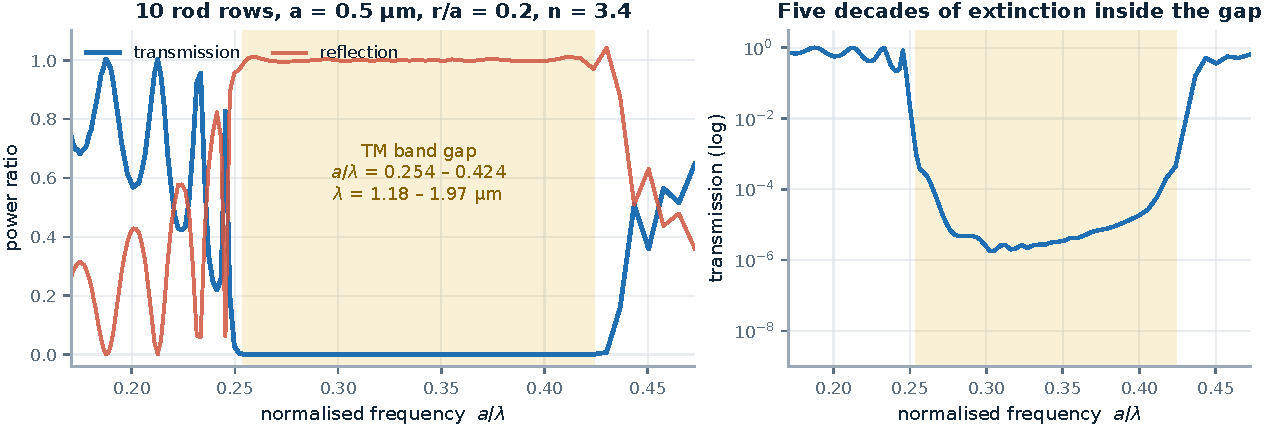
\includegraphics[width=.95\textwidth]{figures/field-phc-gap.pdf}
  \end{center}
  \vspace{-1mm}
  \begin{columns}[T]
    \begin{column}{.66\textwidth}
      \footnotesize
      정사각 격자 유전체 rod ($a=0.5$ µm, $r/a=0.2$, $n=3.4$) 10열, TM 편광.
      broadband one-way 평면 소스 + 주기 경계 + flux 모니터, 공기 reference로 정규화.
    \end{column}
    \begin{column}{.3\textwidth}
      \caveat{CPU float64로 두 번(구조/reference) 실행해 약 25초. GPU에서는 이보다 훨씬 짧습니다.}
    \end{column}
  \end{columns}
\end{frame}

\begin{frame}{우리 연구 대상으로 직접 계산 2: W1 선결함 도파로}
  \begin{columns}[T]
    \begin{column}{.62\textwidth}
      \begin{center}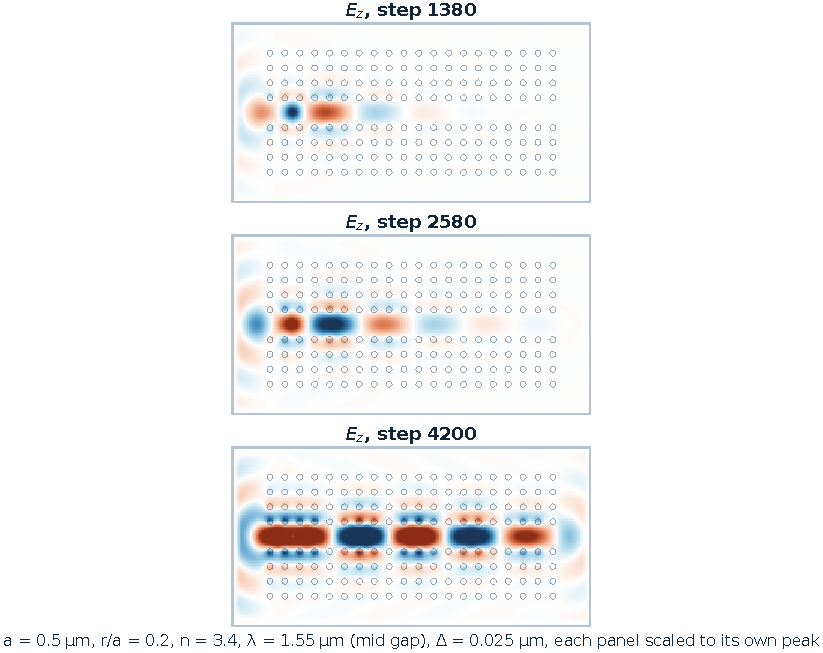
\includegraphics[width=\textwidth]{figures/field-phc-w1.pdf}\end{center}
    \end{column}
    \begin{column}{.36\textwidth}
      \begin{itemize}\footnotesize
        \item 같은 결정에서 한 줄을 제거한 W1 채널
        \item 밴드갭 안쪽 1.55 µm ($a/\lambda = 0.32$)로 여기
        \item 결정 안쪽으로는 evanescent, 채널을 따라 전파
        \item 160개 rod · 480$\times$240 격자 · 6000 스텝을 CPU에서 약 20초
      \end{itemize}
      \vspace{2mm}
      \begin{block}{\footnotesize 의미}
        \footnotesize 랩에서 쓰는 PhC/metasurface 구조를 그대로 올려서, 스펙트럼과 필드를 같은 도구에서 얻습니다.
      \end{block}
    \end{column}
  \end{columns}
\end{frame}

\begin{frame}{필드 시각화 예: 도파로와 산란체}
  \begin{center}
    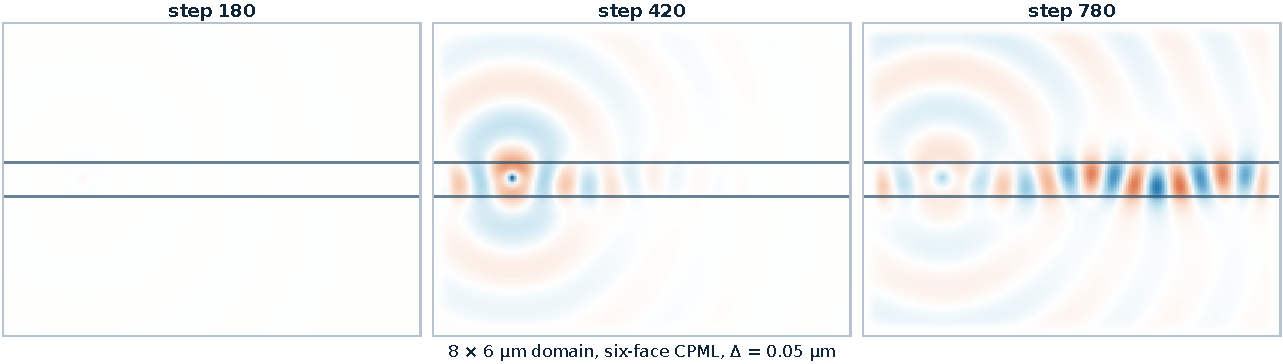
\includegraphics[width=.82\textwidth]{figures/field-waveguide.pdf}\\[-1mm]
    \caveat{SiN 도파로, 다이폴 여기, 6면 CPML — 같은 계산이 UI의 Field visualizer에서 애니메이션으로 재생됩니다.}\\[2mm]
    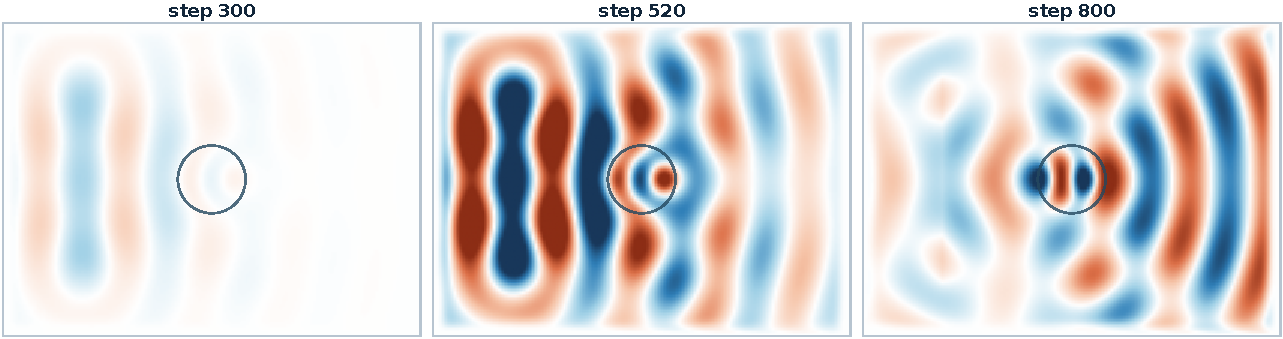
\includegraphics[width=.82\textwidth]{figures/field-scatterer.pdf}\\[-1mm]
    \caveat{유전체 원기둥에 평면파 입사. 모든 그림은 이 저장소의 네이티브 솔버가 계산한 실제 $E_z$ 스냅샷입니다.}
  \end{center}
\end{frame}

% ===========================================================================
\section{성능}
% ===========================================================================

\begin{frame}{Lumerical FDTD와의 기록된 비교}
  \begin{center}
    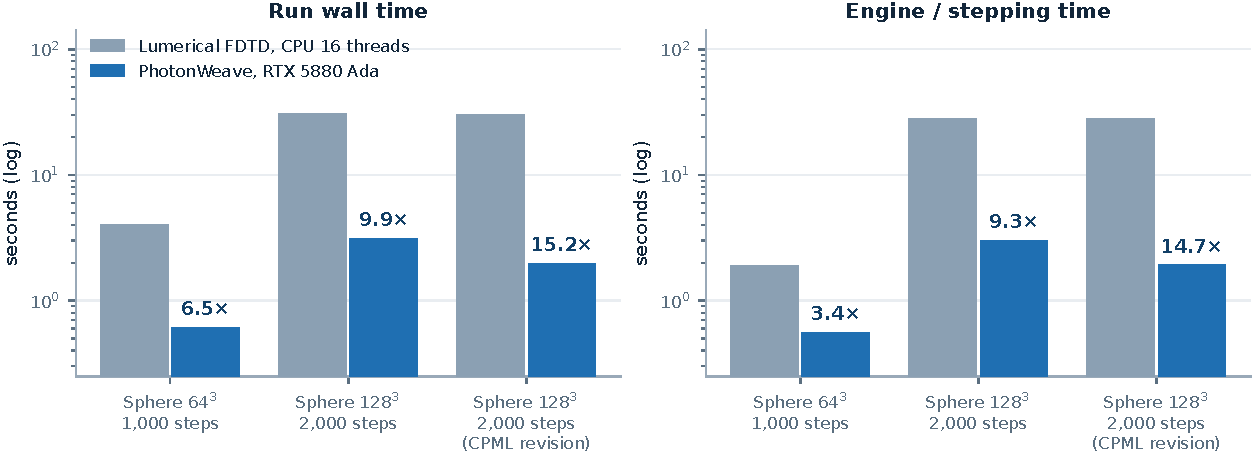
\includegraphics[width=.92\textwidth]{figures/chart-lumerical.pdf}
  \end{center}
  \vspace{-2mm}
  \begin{columns}[T]
    \begin{column}{.55\textwidth}
      \footnotesize
      6 µm 정육면체 도메인의 $n=2$ 구(반지름 0.6 µm), 1.55 µm Gaussian dipole, 포인트 모니터 1개.
      각 값은 3회 측정의 중앙값입니다.
    \end{column}
    \begin{column}{.42\textwidth}
      \begin{block}{\footnotesize 이 표를 읽는 법}
        \scriptsize
        \textcolor{pwred}{과거 빌드의 기록}이며 현재 릴리스의 검증된 speedup이 아닙니다.
        dipole 정규화·필드 보간·흡수 경계가 달라 \textcolor{pwred}{동일 정확도 비교가 아니고},
        Lumerical GPU 엔진과는 측정하지 않았습니다.
      \end{block}
    \end{column}
  \end{columns}
\end{frame}

\begin{frame}{그래서 지금 다시 해야 하는 비교}
  \begin{center}
    \small
    \begin{tabular}{p{7.4cm} l}
      \toprule
      \textbf{필요한 비교} & \textbf{현재 상태} \\
      \midrule
      현재 PhotonWeave vs Lumerical CPU, 공통 정확도 목표 & \textcolor{pwred}{새 matched validation 필요} \\
      현재 PhotonWeave vs Lumerical GPU, 같은 RTX 5880 & \textcolor{pwred}{미측정} \\
      다구조 배치 / 역설계 throughput vs Lumerical & \textcolor{pwred}{미측정} \\
      \midrule
      오픈소스 GPU 기준선(flaport/fdtd + CUDA Graph) 대비 & \textcolor{pwgreen}{측정 완료} \\
      네이티브 CPU vs GPU, 동일 코드 경로 & \textcolor{pwgreen}{측정 완료} \\
      해석해(박막, Mie) 대비 정확도 & \textcolor{pwgreen}{측정 완료, 한계 명시} \\
      \bottomrule
    \end{tabular}
  \end{center}
  \vspace{2mm}
  \begin{columns}[T]
    \begin{column}{.6\textwidth}
      \footnotesize 랩미팅에서 주장하는 범위: \hl{"같은 물리 설정에서 우리 GPU 경로가 우리 CPU 경로와 공개 GPU 기준선보다 빠르다"}.
    \end{column}
    \begin{column}{.36\textwidth}
      \caveat{상용 솔버 대비 "동일 정확도 speedup"은 아직 주장하지 않습니다.}
    \end{column}
  \end{columns}
\end{frame}

\begin{frame}{오픈소스 GPU 기준선 대비 단일 케이스}
  \begin{center}
    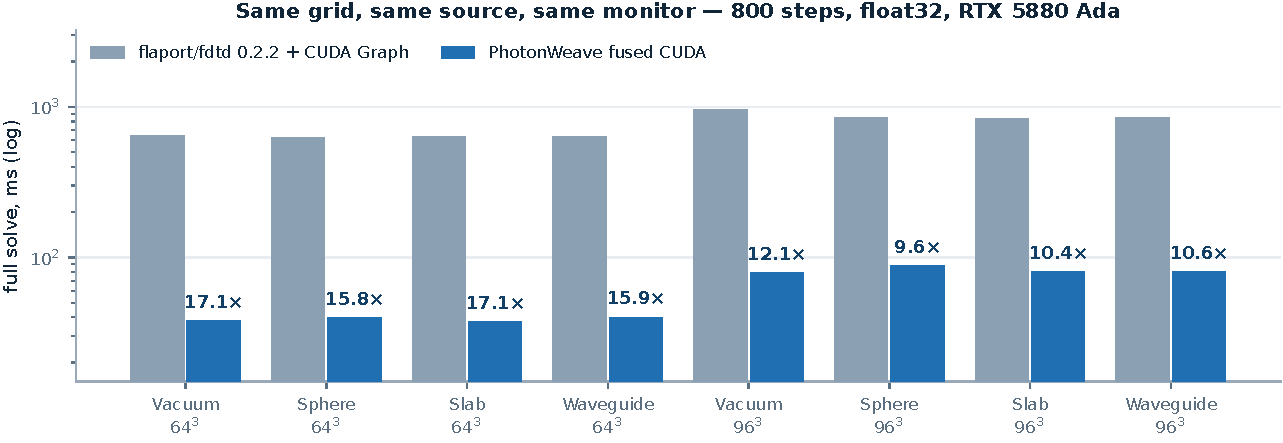
\includegraphics[width=.95\textwidth]{figures/chart-flaport.pdf}
  \end{center}
  \vspace{-1mm}
  \begin{columns}[T]
    \begin{column}{.63\textwidth}
      \footnotesize
      두 엔진에 \hl{동일한 voxel 유전율·시간 스텝·샘플 소스·포인트 모니터}를 주고,
      상용 기준선이 아닌 공개 코드에 CUDA Graph 어댑터까지 붙여 준 비교입니다.
      8개 케이스 모두 포인트 트레이스 상대 L2 \num{$<$0.04\%}.
    \end{column}
    \begin{column}{.34\textwidth}
      \caveat{최종 full field는 상위 PML 스텐실 차이로 동일하지 않습니다. 원자료에 오차를 모두 남겨 두었습니다.}
    \end{column}
  \end{columns}
\end{frame}

\begin{frame}{배치: 같은 문제를 CPU와 GPU로}
  \begin{columns}[T]
    \begin{column}{.46\textwidth}
      \begin{center}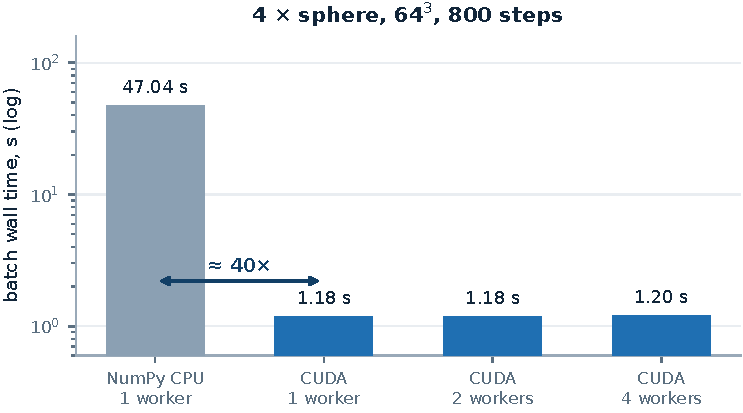
\includegraphics[width=\textwidth]{figures/chart-cpu-gpu.pdf}\end{center}
      \caveat{4개 독립 구 케이스, 64$^3$, 800 스텝. 워커를 2/4개로 늘려도 이 문제에서는 더 빨라지지 않습니다.}
    \end{column}
    \begin{column}{.5\textwidth}
      \begin{center}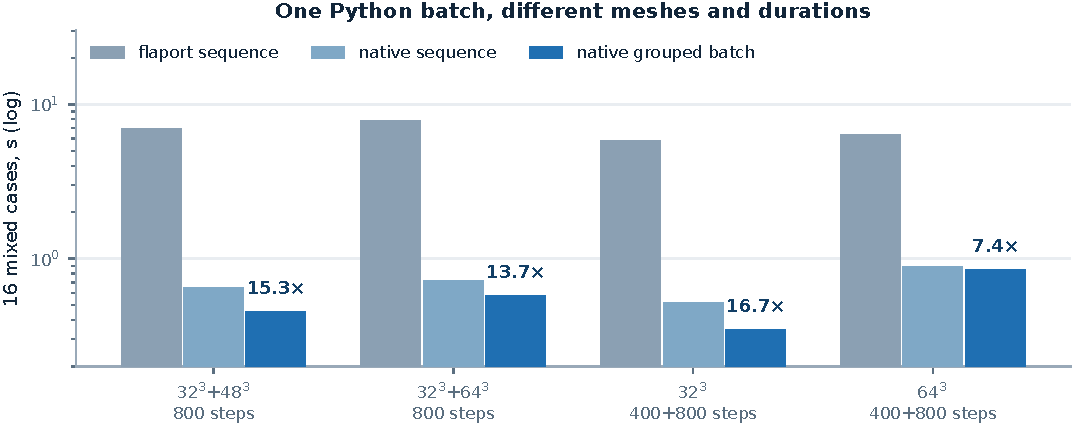
\includegraphics[width=\textwidth]{figures/chart-grouped.pdf}\end{center}
      \caveat{메시와 지속시간이 섞인 16 케이스를 한 Python 배치로. 호환 케이스를 자동 그룹화하고 입력 순서로 결과를 복원합니다.}
    \end{column}
  \end{columns}
\end{frame}

\begin{frame}{배치 축의 한계도 같이 봅니다}
  \begin{columns}[T]
    \begin{column}{.5\textwidth}
      \begin{center}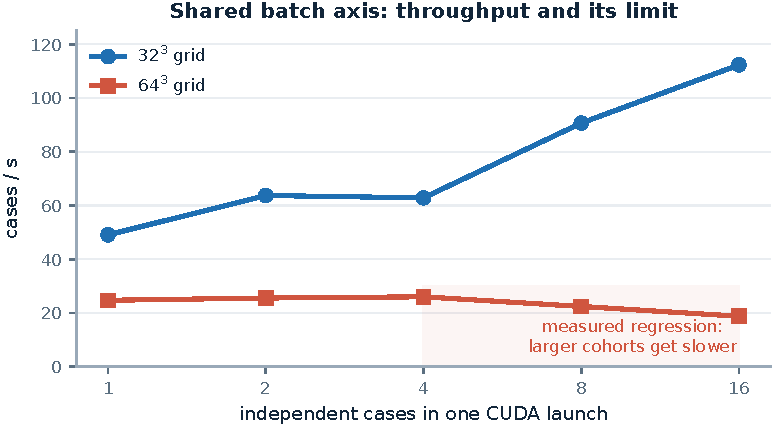
\includegraphics[width=\textwidth]{figures/chart-batch-scaling.pdf}\end{center}
    \end{column}
    \begin{column}{.46\textwidth}
      \begin{itemize}\footnotesize
        \item 32$^3$에서는 16 케이스까지 throughput이 증가 (\num{112 cases/s})
        \item 64$^3$에서는 8, 16 케이스에서 \alert{오히려 느려짐}
        \item 해결책: \texttt{cohort\_size}로 한 번에 묶는 케이스 수를 제한
        \item \texttt{tune\_tensor\_batch()}가 실제 측정으로 크기를 고르지만, \hl{튜닝 자체가 비용}
        \item 64$^3$에서는 튜닝 비용을 회수하는 데 같은 앙상블 144--420회가 필요
      \end{itemize}
      \source{README.md · ensembles.json}
    \end{column}
  \end{columns}
\end{frame}

\begin{frame}{시간이 실제로 줄어든 곳}
  \begin{center}
    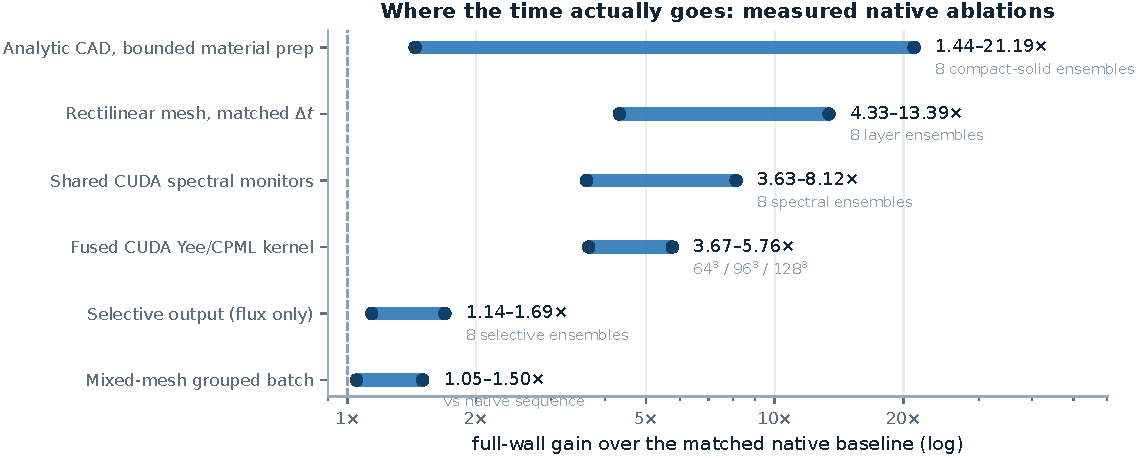
\includegraphics[width=.9\textwidth]{figures/chart-ablation.pdf}
  \end{center}
  \vspace{-1mm}
  \footnotesize
  단일 커널 최적화만이 아니라, \hl{호스트 준비 시간·불필요한 셀·저장하지 않아도 되는 출력}을 제거한 것이
  실제 워크플로 시간에 더 크게 기여했습니다. 모든 행은 동일 조건의 네이티브 baseline과 비교한 full-wall 시간입니다.
\end{frame}

% ===========================================================================
\section{미분 가능 FDTD와 역설계}
% ===========================================================================

\begin{frame}{왜 adjoint인가}
  \begin{center}
    \begin{tikzpicture}[font=\scriptsize,
      st/.style={draw=pwblue, fill=pwblue!10, rounded corners=2pt, minimum width=1.05cm, minimum height=.6cm},
      ck/.style={draw=pwamber, fill=pwamber!20, rounded corners=2pt, minimum width=1.05cm, minimum height=.6cm},
      ad/.style={draw=pwred, fill=pwred!10, rounded corners=2pt, minimum width=1.05cm, minimum height=.6cm}]
      \node[align=right, text width=1.9cm] at (-1.9,1.0) {\textbf{forward}\\$\mathbf{E},\mathbf{H}$};
      \foreach \i in {0,...,7} {
        \ifnum\i=0 \node[ck] (f\i) at (\i*1.3,1.0) {} ;
        \else\ifnum\i=4 \node[ck] (f\i) at (\i*1.3,1.0) {};
        \else \node[st] (f\i) at (\i*1.3,1.0) {}; \fi\fi}
      \foreach \i [evaluate=\i as \j using int(\i+1)] in {0,...,6} \draw[-Stealth, pwdeep] (f\i)--(f\j);
      \node[right=2mm of f7, text width=2.4cm] {목적함수 $f$\\(스펙트럼 / flux / 전자수)};

      \node[align=right, text width=1.9cm] at (-1.9,-1.0) {\textbf{backward}\\$\lambda$};
      \foreach \i in {0,...,7} \node[ad] (b\i) at (\i*1.3,-1.0) {};
      \foreach \i [evaluate=\i as \j using int(\i+1)] in {0,...,6} \draw[Stealth-, pwred] (b\i)--(b\j);
      \draw[-Stealth, pwred] (f7.south) -- (b7.north);

      \draw[-Stealth, pwamber, thick] (f0.south) to[out=-60,in=120] node[left, pwamber!80!black, font=\tiny] {replay} (b1.north west);
      \draw[-Stealth, pwamber, thick] (f4.south) to[out=-60,in=120] (b5.north west);
      \node[pwamber!80!black, font=\tiny, above] at (0,1.45) {checkpoint};
      \node[pwamber!80!black, font=\tiny, above] at (5.2,1.45) {checkpoint};
    \end{tikzpicture}
  \end{center}
  \vspace{1mm}
  \begin{columns}[T]
    \begin{column}{.48\textwidth}
      \begin{itemize}\footnotesize
        \item 파라미터가 $P$개여도 기울기 1회 = forward 1회 + backward 1회
        \item 유한차분 스윕은 $P+1$회 계산 필요
        \item 전체 시간 이력 저장 대신 \hl{checkpoint replay}로 메모리 제한
      \end{itemize}
    \end{column}
    \begin{column}{.48\textwidth}
      \begin{block}{\footnotesize 현재 미분 가능한 것}
        \footnotesize 대각 $\varepsilon$, Torch geometry map, 고정 실수/Bloch 경계,
        Drude/Lorentz 파라미터($\varepsilon_\infty$, 진동자 세기, 공명, damping),
        포인트 신호 · 스펙트럼 · 고정 검출 평면
      \end{block}
    \end{column}
  \end{columns}
\end{frame}

\begin{frame}{adjoint 1회 비용: CPU vs GPU}
  \begin{center}
    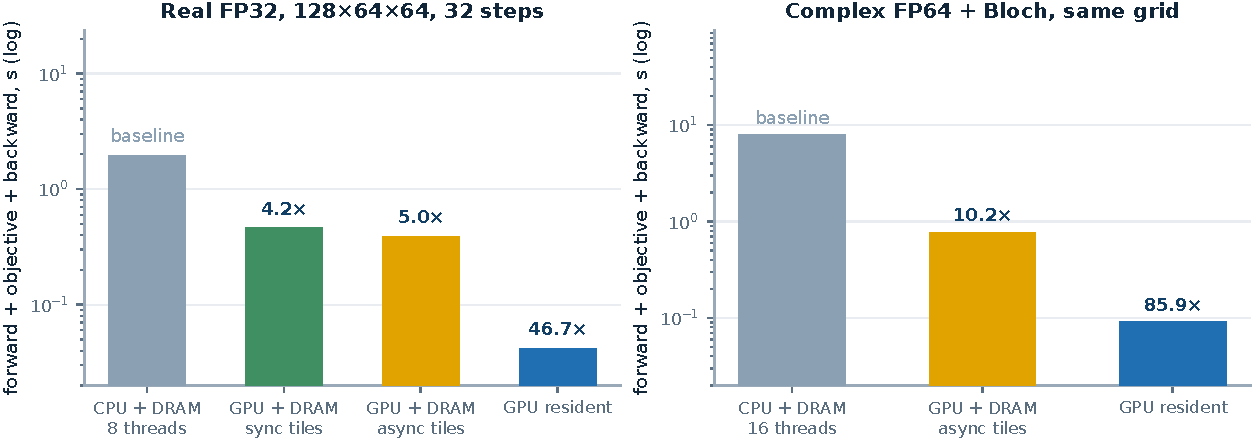
\includegraphics[width=.92\textwidth]{figures/chart-adjoint.pdf}
  \end{center}
  \vspace{-1mm}
  \footnotesize
  같은 코드 경로, 같은 격자(128$\times$64$\times$64, 32 스텝), forward + 목적함수 + backward 전체 시간.
  모든 모드가 신호·기울기 검사를 통과했고, CPU는 1/4/8/16 스레드 중 가장 빠른 설정을 사용했습니다.
  \caveat{이 문제는 VRAM 안에 들어갑니다. 48 GB를 넘는 영역의 속도나 외부 솔버 성능을 말하는 수치가 아닙니다.}
\end{frame}

\begin{frame}{VRAM보다 큰 문제를 푸는 방법}
  \begin{columns}[T]
    \begin{column}{.47\textwidth}
      \begin{center}
        \begin{tikzpicture}[font=\scriptsize,
          tier/.style={draw=pwgrey, rounded corners=2pt, minimum width=4.6cm, minimum height=.95cm, align=center}]
          \node[tier, fill=pwblue!12, draw=pwblue] (v) at (0,2.1) {\textbf{VRAM (48 GB)}\\현재 타일 + 실행 버퍼};
          \node[tier, fill=pwgreen!10, draw=pwgreen] (d) at (0,.85) {\textbf{DRAM 뱅크}\\전체 E/H · ADE 상태};
          \node[tier, fill=pwamber!12, draw=pwamber] (f) at (0,-.4) {\textbf{파일 백킹 (NVMe)}\\더 큰 상태, 실험적};
          \draw[-Stealth, pwdeep] (v.west) to[out=180, in=180] node[left, font=\tiny] {tile out} (d.west);
          \draw[-Stealth, pwdeep] (d.east) to[out=0, in=0] node[right, font=\tiny] {tile in} (v.east);
          \draw[-Stealth, pwgrey] (d.south)--(f.north);
          \node[align=center, font=\tiny, text width=5cm] at (0,-1.5) {space-time tile: 한 칸 Yee 의존 cone을\\halo로 포함해 손실 없이 분할};
        \end{tikzpicture}
      \end{center}
    \end{column}
    \begin{column}{.49\textwidth}
      \begin{center}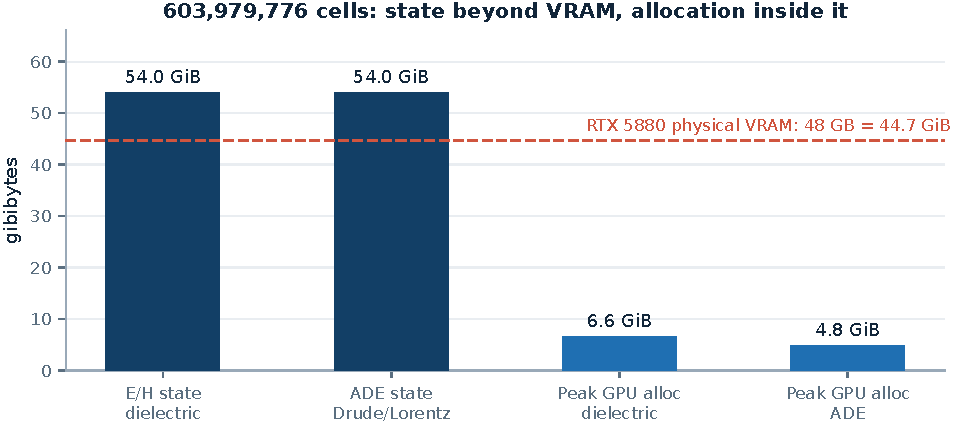
\includegraphics[width=\textwidth]{figures/chart-beyond-vram.pdf}\end{center}
      \vspace{1mm}
      \footnotesize
      603,979,776 셀, E/H 54 GiB 상태에서 \hl{10 스텝 전진 + 1차 기울기} 검증 완료
      (peak GPU 할당 6.6 GiB = 7.09 GB, 52분). 분산재료 ADE 버전은 4.8 GiB, 54.8분.
      \caveat{용량 증명이지 속도 우위가 아닙니다. 실제 응용 지속시간에서의 성능은 미검증.}
    \end{column}
  \end{columns}
\end{frame}

\begin{frame}{분산 재료(Drude/Lorentz)까지 미분}
  \begin{center}
    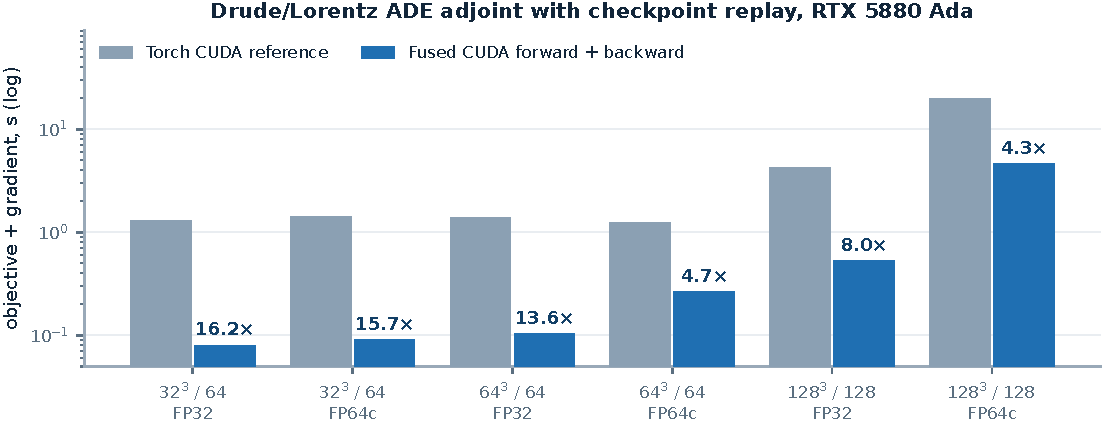
\includegraphics[width=.92\textwidth]{figures/chart-dispersive.pdf}
  \end{center}
  \vspace{-1mm}
  \begin{columns}[T]
    \begin{column}{.62\textwidth}
      \footnotesize
      ADE의 P/Q 상태까지 checkpoint replay에 포함하고, 재료 기울기는 atomics 없이 블록 리덕션으로 모읍니다.
      공유 파라미터는 compact하게 유지되어 극점 수가 늘어도 메모리가 선형 증가하지 않습니다.
    \end{column}
    \begin{column}{.34\textwidth}
      \caveat{같은 연산(전진+목적함수+역전파)을 우리 Torch 경로와 비교한 내부 측정입니다.}
    \end{column}
  \end{columns}
\end{frame}

\begin{frame}[fragile]{설계 루프: 지금 돌아가는 형태}
  \begin{columns}[T]
    \begin{column}{.46\textwidth}
      \begin{center}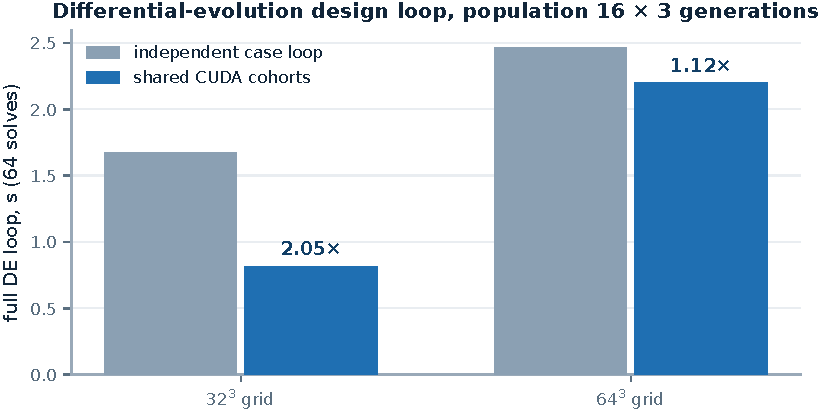
\includegraphics[width=\textwidth]{figures/chart-design-loop.pdf}\end{center}
      \caveat{블랙박스(미분 없는) differential evolution 루프. population 16 $\times$ 3세대 = 64회 forward.}
    \end{column}
    \begin{column}{.5\textwidth}
\begin{lstlisting}[basicstyle=\ttfamily\tiny]
import torch
from photonweave import (DifferentiableSimulation,
    AdjointOptions, smooth_sphere_epsilon)

model = DifferentiableSimulation(project,
    AdjointOptions(checkpoints=4, storage="host"))
radius = torch.nn.Parameter(
    torch.tensor(0.25, dtype=torch.float64))
opt = torch.optim.Adam([radius], lr=0.003)

for step in range(iterations):
    opt.zero_grad()
    epsilon = smooth_sphere_epsilon(
        project.region, radius, width=0.09, inside=3.0)
    result = model(epsilon)             # forward
    loss = result.signals[:, 0].abs().square().mean()
    loss.backward()                     # discrete adjoint
    opt.step()
\end{lstlisting}
      \vspace{1mm}
      \caveat{\texttt{examples/differentiable\_design.py}의 실제 코드. 스트리밍 실행은 \texttt{StreamedSimulation}으로 같은 자리에 들어갑니다. 포트 정규화 목적함수 검증은 진행 중입니다.}
    \end{column}
  \end{columns}
\end{frame}

% ===========================================================================
\section{상호운용, 현황, 다음 단계}
% ===========================================================================

\begin{frame}{기존 .fsp 자산을 버리지 않기}
  \begin{center}
    \begin{tikzpicture}[font=\scriptsize,
      blk/.style={draw=pwgrey, fill=white, rounded corners=2pt, inner sep=5pt, align=center, text width=2.8cm}]
      \node[blk, draw=pwdeep] (fsp) at (0,0) {\textbf{.fsp 파일}\\(벤더 런타임 없이 독립 파싱)};
      \node[blk] (scene) at (3.9,0) {인식된 레코드\\구조 · 소스 · 모니터 · 메시};
      \node[blk, draw=pwblue, fill=pwblue!8] (gpu) at (7.8,0) {PhotonWeave\\프로젝트 모델};
      \node[blk, draw=pwgreen, fill=pwgreen!8] (run) at (11.4,0) {GPU 실행\\결과};
      \draw[-Stealth, pwdeep] (fsp)--(scene); \draw[-Stealth, pwdeep] (scene)--(gpu); \draw[-Stealth, pwdeep] (gpu)--(run);
      \draw[-Stealth, pwamber, thick] (gpu.south) to[out=-90, in=-90] node[below, font=\tiny, pwamber!80!black] {writeback: 편집하지 않은 바이트는 보존} (fsp.south);
    \end{tikzpicture}
  \end{center}
  \vspace{1mm}
  \begin{columns}[T]
    \begin{column}{.55\textwidth}
      \begin{itemize}\footnotesize
        \item box, 회전 타원체/원기둥, 부분 링, 단순 polygon extrusion import
        \item 메시 간격·span·CAD/PML 경계·CFL, 소스 대역/위상, 모니터 스펙트럼 writeback
        \item primitive 추가/삭제/복제/재정렬, 소스·모니터 리스트 편집
      \end{itemize}
    \end{column}
    \begin{column}{.42\textwidth}
      \caveat{지원하지 않는 물리는 변환을 막습니다. 외부 도구의 새 레코드 수용·그룹·결과 포함 파일·일반 호환성은 미해결.}
    \end{column}
  \end{columns}
\end{frame}

\begin{frame}{오픈소스 GPU FDTD 지형에서의 위치}
  \begin{center}\scriptsize
    \begin{tabular}{l p{2.2cm} p{2.6cm} p{2.4cm} p{2.4cm}}
      \toprule
      & \textbf{백엔드} & \textbf{동일 GPU 배치} & \textbf{adjoint} & \textbf{비고} \\
      \midrule
      \textbf{PhotonWeave} & PyTorch + native CUDA & 공유 CUDA launch, cohort 분할, 측정 기반 선택 & 부분: 실수 유전체 Yee/CPML + 분산 파라미터 & 브라우저 CAD, FSP 서브셋, 멀티폴 ADE \\
      FDTDX & JAX & JAX 조합 & \textcolor{pwgreen}{있음} (reversible/checkpoint) & \textcolor{pwred}{역설계는 우리보다 앞섬} \\
      fdtdz & JAX + 전용 CUDA & 미검증 & 등록된 VJP 규칙 없음 & 매우 빠른 전용 범위, z 크기 제약 \\
      flaport/fdtd & NumPy / PyTorch & 공개 Grid는 1 케이스 & 기본 백엔드는 grad 비활성 & 우리가 기반으로 사용·출처 표기 \\
      fdtd3d & C++/CUDA/MPI & 단일 문제 도메인 분할 & 문서화 없음 & \textcolor{pwred}{단일 격자 MPI는 우리에게 없음} \\
      \bottomrule
    \end{tabular}
  \end{center}
  \vspace{2mm}
  \footnotesize
  \hl{정직하게}: FDTDX, fdtdz, fdtd3d와는 같은 GPU에서 속도를 측정하지 못했습니다(현재 워크스테이션에 Linux CUDA 환경 부재).
  기능 차이는 속도 우위가 아닙니다.
\end{frame}

\begin{frame}{아직 안 되는 것 (질문 받기 전에 먼저)}
  \begin{columns}[T]
    \begin{column}{.48\textwidth}
      \textbf{물리}
      \begin{itemize}\footnotesize
        \item 이득 매질, 비선형, 이방성 미지원
        \item 대칭/반대칭 경계, PEC/PMC 미구현
        \item 경사 입사 one-way/TFSF, 도파로 모드 소스 미구현
        \item far-field 변환, mode port, S-parameter 미구현
        \item conformal/subpixel은 실험적 (기본은 staircase)
      \end{itemize}
    \end{column}
    \begin{column}{.48\textwidth}
      \textbf{워크플로 · 검증}
      \begin{itemize}\footnotesize
        \item 체크리스트 1,661행 중 구현 160 / 부분 231 / 미구현·미검증 1,270 \\ \caveat{(속성 수이며 제품 완성도 비율이 아님)}
        \item 단일 격자 MPI 분할 없음
        \item 응용 수준 역설계(mode/port 정규화 목적함수) 검증 미완료
        \item 상용 솔버와 동일 정확도 조건의 재측정 필요
        \item 공개 배포는 라이선스 검토 미완료
      \end{itemize}
    \end{column}
  \end{columns}
  \vspace{2mm}
  \caveat{문서: docs/FEATURE\_CHECKLIST.md · docs/PARITY\_ROADMAP.md · docs/RELEASE\_REVIEW.md}
\end{frame}

\begin{frame}{다음 단계}
  \begin{columns}[T]
    \begin{column}{.32\textwidth}
      \begin{block}{\footnotesize 단기}
        \footnotesize
        \begin{itemize}
          \item 동일 정확도 기준의 상용 솔버 재측정
          \item mode/port 정규화 목적함수
          \item subpixel 정확도 정리
        \end{itemize}
      \end{block}
    \end{column}
    \begin{column}{.32\textwidth}
      \begin{block}{\footnotesize 중기}
        \footnotesize
        \begin{itemize}
          \item 전 물리 미분 가능화(분산·경계 포함)
          \item 통합 메모리 정책 (resident/streamed 자동 선택)
          \item 실제 응용 지속시간의 대형 역설계
        \end{itemize}
      \end{block}
    \end{column}
    \begin{column}{.32\textwidth}
      \begin{block}{\footnotesize 랩 적용}
        \footnotesize
        \begin{itemize}
          \item PhC/metasurface 스윕을 배치로 이전
          \item 측정 n/k 데이터 피팅 후 프로젝트에 보관
          \item GPU 워크스테이션에 SSH 터널로 공유 사용
        \end{itemize}
      \end{block}
    \end{column}
  \end{columns}
  \vspace{3mm}
  \begin{center}
    \small 필요한 구조·조건을 알려주시면 그 케이스로 먼저 벤치마크하고, 정확도 게이트를 붙여서 가져오겠습니다.
  \end{center}
\end{frame}

\begin{frame}[standout]
  요약\\[4mm]
  {\normalsize
  \begin{minipage}{.8\textwidth}
    \begin{itemize}
      \item 상용 FDTD와 같은 작업 순서를 유지한 \textbf{브라우저 + Python 워크벤치}
      \item 같은 물리 설정에서 우리 CPU 경로와 공개 GPU 기준선보다 \textbf{빠른 CUDA 엔진}
      \item 설계 루프를 위한 \textbf{배치 실행과 discrete adjoint}, VRAM을 넘는 메모리 계층
      \item 속도 수치는 조건과 한계를 함께 기록 — 상용 솔버 동일정확도 비교는 \textbf{진행 중}
    \end{itemize}
  \end{minipage}}
\end{frame}

% ===========================================================================
\appendix

\begin{frame}{백업: 수치 규약}
  \begin{columns}[T]
    \begin{column}{.48\textwidth}
      \begin{itemize}\footnotesize
        \item 길이·파장은 µm, API 시간 배열은 초
        \item 진폭은 reduced field (보정된 V/m 아님)
        \item E와 H는 시공간에서 엇갈려 있으므로 곧바로 곱해 Poynting으로 쓰지 않음
        \item 포인트 모니터: FFT bin 또는 사용자 지정 범위 DFT, None/Start/End/Full/Hann apodization
        \item 평면 모니터: 6성분 복소장 + 부호 있는 flux, reference 정규화 필요
      \end{itemize}
    \end{column}
    \begin{column}{.48\textwidth}
      \begin{itemize}\footnotesize
        \item 재료: 상수 $n \geq 1$, 수동 등방 Drude/Lorentz 최대 16 극점
        \item 내장 Si/SiN/SiO$_2$ 값은 편집 가능한 근사치이며 광학상수 DB가 아님
        \item 측정 n/k 샘플을 수동 극점으로 피팅하고 오차를 명시
        \item 모든 벤치마크는 3회 반복 중앙값, warmup 후 측정, cold compile 제외
        \item 3회 반복은 신뢰구간을 주지 않음
      \end{itemize}
    \end{column}
  \end{columns}
\end{frame}

\begin{frame}[fragile]{백업: 이 슬라이드의 그림을 다시 만드는 법}
  \begin{columns}[T]
    \begin{column}{.56\textwidth}
\begin{lstlisting}[language=bash]
# figures: charts + real CPU simulations
python docs/presentation/make_figures.py

# slides (XeLaTeX, Korean)
cd docs/presentation
xelatex photonweave-lab-meeting.tex

# or
bash docs/presentation/build.sh
\end{lstlisting}
    \end{column}
    \begin{column}{.42\textwidth}
      \footnotesize
      \begin{itemize}
        \item 필드 그림 4종은 실행 때마다 \hl{실제로 다시 계산}됩니다 (CPU, 총 1분 이내)
        \item 성능 차트의 모든 수치는 README와 docs/validation의 기록값
        \item UI 화면은 로컬 서버(\texttt{python -m photonweave.cli serve})의 실제 캡처
      \end{itemize}
    \end{column}
  \end{columns}
\end{frame}

\begin{frame}{백업: 측정 환경}
  \begin{center}\small
    \begin{tabular}{l l}
      \toprule
      GPU 측정 & NVIDIA RTX 5880 Ada Generation 48 GB, Windows, PyTorch 2.10 \\
      보조 GPU & RTX 3060 (복소 FP64 CR 관련 측정) \\
      CPU 비교 & Xeon w3-2435 (8/16 스레드), i7-12700 (8 스레드) \\
      외부 기준선 & flaport/fdtd 0.2.2 + 자체 CUDA Graph 어댑터 + 동일 fused 관측자 \\
      상용 기록 & Lumerical FDTD CPU 1 프로세스 16 스레드, API 버전 문자열 8.31.3633 (v241) \\
      정확도 게이트 & 포인트 트레이스 1\%, flux 2\%, 복소 평면 DFT 1\% (외부), 네이티브 간 bitwise \\
      \bottomrule
    \end{tabular}
  \end{center}
  \vspace{3mm}
  \caveat{Lumerical 계산 결과·필드·프로젝트 파일은 저장소에 포함하지 않으며, 타이밍 요약만 기록했습니다. 해당 표는 공개 배포 전 라이선스 검토 대상입니다.}
\end{frame}

\end{document}
